%ajouter draft pour voir débordement

%%%%%

\documentclass[12pt,french]{article}


\usepackage[utf8]{inputenc}
\usepackage[T1]{fontenc}
\usepackage{lmodern}
%règles mes marges et format papier
\usepackage{geometry} %modif marge et formet
\geometry{left=3cm,right=2cm,top=2.5cm,bottom=2.5cm}
\usepackage{amsmath, amssymb, amsthm}
\usepackage{fancyhdr} %pour les entêtes et bas de page
\usepackage{lastpage} %pour numéroter les pages charge la derniere page
\usepackage{graphicx} %pour inclure des img
\usepackage{dsfont}
\usepackage{float} %pour le placement des figures
\usepackage{hyperref} %pour mettre des liens hypertext
\usepackage{calc} %permet de calculer les marges pour encadrer les textes
\usepackage{color, xcolor} %gère les couleurs
\usepackage{listings} %pour afficher le code annexe


%glossaire
\usepackage[acronym]{glossaries}
\makeglossaries

\newglossaryentry{chiffre}
{
	name=chiffré,
	description={Le chiffrage est une technique de protection de données sensibles par le biais d'un algorithme de chiffrement. Cette technique est utilisée pour sécuriser les informations confidentielles en les transformant en un code illisible pour une personne non autorisée.}
}

\newglossaryentry{API}
{
	name=API,
	description={L'API (Application Programming Interface) est un ensemble de protocoles et d'outils permettant à différents logiciels de communiquer entre eux. Elle permet à des développeurs d'utiliser les fonctionnalités d'un logiciel tiers dans leur propre application.}
}

\newglossaryentry{SACEM}
{
	name=SACEM,
	description={La SACEM (Société des Auteurs, Compositeurs et Éditeurs de Musique) est une société française de gestion des droits d'auteur. Elle a pour mission de collecter et de répartir les droits d'auteur aux auteurs, compositeurs et éditeurs de musique.}
}

\newglossaryentry{Open-source}
{
	name=Open-source,
	description={Le terme open-source désigne un logiciel dont le code source est accessible publiquement. Il peut être utilisé, modifié et distribué librement par les utilisateurs, contrairement aux logiciels propriétaires.}
}

\newglossaryentry{Front}
{
	name=Front,
	description={En développement web, la notion de "front end" fait référence à l’ensemble des éléments visibles et accessibles directement sur un site web (voire sur une application web ou une application web mobile)}
}


\newglossaryentry{Back}
{
	name=Back,
	description={Le "back end" concerne toute la partie invisible de la conception d’un site internet, tel que le développement de bases de données, par exemple.
	}
}


\newglossaryentry{Framework}
{
	name=Framework,
	description={Un framework (ou infrastructure logicielle en français ) désigne en programmation informatique un ensemble d'outils et de composants logiciels à la base d'un logiciel ou d'une application.
	}
}

\newglossaryentry{Typescript}
{
	name=Typescript,
	description={TypeScript est un langage de programmation libre et Open-source développé par Microsoft qui a pour but d'améliorer et de sécuriser la production de code JavaScript. Il s'agit d'un sur-ensemble syntaxique strict de JavaScript (c'est-à-dire que tout code JavaScript correct peut être utilisé avec TypeScript).
	}
}

\newglossaryentry{SCSS}
{
	name=SCSS,
	description={Le Sassy CSS ou SCSS est à la fois un langage et une méthode d’utilisation du CSS qui utilise les fonctionnalités de Sass (pré-processeur CSS Syntacticaly Awesome Style Sheet).
	}
}

\newglossaryentry{HTML}
{
	name=HTML,
	description={L'HyperText Markup Language, HTML, désigne un type de langage informatique descriptif. Il s'agit plus précisément d'un format de données utilisé dans l'univers d'Internet pour la mise en forme des pages Web. Il permet, entre autres, d'écrire de l'hypertexte, mais aussi d'introduire des ressources multimédias dans un contenu.
	}
}

\newglossaryentry{Javascript}
{
	name=JavaScript,
	description={JavaScript désigne un langage de développement informatique, et plus précisément un langage de script orienté objet. On le retrouve principalement dans les pages Internet. Il permet, entre autres, d'introduire sur une page web ou HTML des petites animations ou des effets.
	}
}

\newglossaryentry{sprint}
{
	name=sprint,
	description={Le sprint agile est une étape phare de la méthode Agile. Il s’agit d’une période courte délimitée dans le temps, durant laquelle les différents collaborateurs d’un projet vont travailler sur un objectif détaillé et atteignable. Cet objectif permet de faire avancer le projet. 
	}
}

\newglossaryentry{Web scraping}
{
	name=Web scraping,
	description={Le Web scraping (parfois appelé harvesting ou en français moissonage) est une technique d'extraction du contenu de sites Web, via un script ou un programme, dans le but de le transformer pour permettre son utilisation dans un autre contexte comme l'enrichissement de bases de données, le référencement ou l'exploration de données.
	}
}

\newglossaryentry{HTTP}
{
	name=HTTP,
	description={L'http, pour Hypertext Transfer Protocol, désigne dans le langage informatique un protocole de communication entre un client et un serveur pour le World Wide Web. On le traduit littéralement en français par protocole de transfert hypertexte.
	}
}

\newglossaryentry{sale}
{
	name=salé,
	description={Le salage est une méthode permettant de renforcer la sécurité des informations qui sont destinées à être hachées (par exemple des mots de passe) en y ajoutant une donnée supplémentaire afin d’empêcher que deux informations identiques ne conduisent à la même empreinte 
	}
}

\newglossaryentry{CSS}
{
	name=CSS,
	description={Le CSS est un langage informatique utilisé sur Internet pour la mise en forme de fichiers et de pages HTML. On le traduit en français par feuilles de style en cascade.
	}
}

\newglossaryentry{SQL}
{
	name=SQL,
	description={Le langage SQL (Structured Query Language) est un langage informatique utilisé pour exploiter des bases de données. Il permet de façon générale la définition, la manipulation et le contrôle de sécurité de données.
	}
}

\newglossaryentry{token}
{
	name=token,
	description={En français "jeton". L’authentification par jeton est une forme d’authentification qui permet à un utilisateur d’accéder à un service en ligne, une application, ou un site web sans qu’il n’ait à ressaisir ses identifiants. Par conséquent, grâce à cette forme d’authentification, l’utilisateur pourra accéder à ses ressources en ligne, au moyen de ce jeton d’accès, tant qu’il reste valide.
	}
}
%% a faire
\newglossaryentry{table}
{
	name=table,
	description={Dans les bases de données relationnelles, une table est un ensemble de données organisées sous forme d'un tableau où les colonnes correspondent à des catégories d'information (une colonne peut stocker des numéros de téléphone, une autre des noms...) et les lignes à des enregistrements, également appelés entrées.
	}
}

\newglossaryentry{colonne}
{
	name=colonne,
	description={Dans les bases de données relationnelles, une colonne correspond à un attribut d'une table. Par exemple, dans notre table "MUSIC", les colonnes sont "musicName", "artist" et "idMusic".
	}
}

\newglossaryentry{cle}
{
	name=clé,
	description={Dans les bases de données relationnelles, une clé est un attribut de table qui doit être unique. Si cette clé est primaire, elle permet d'identifier dans une table un élément par rapport au autre. Si elle est secondaire, elle permet de faire le lien entre différentes tables.
	}
}

\newglossaryentry{header}
{
	name=header,
	description={Le terme header se traduit en français par en-tête. Sur une page Web, le header se résume à la partie haute du site, là où apparaît la plupart du temps le titre du site Web et les élements de naviguation.
	}
}



%pour afficher le code de manière esthétique
\lstset{
  aboveskip=3mm,
  belowskip=-2mm,
  backgroundcolor=\color{white},
  basicstyle=\footnotesize,
  breakatwhitespace=false,
  breaklines=true,
  captionpos=b,
  commentstyle=\color{red},
  deletekeywords={...},
  escapeinside={\%*}{*)},
  extendedchars=true,
  framexleftmargin=16pt,
  framextopmargin=3pt,
  framexbottommargin=6pt,
  frame=tb,
  keepspaces=true,
  keywordstyle=\color{blue},
  language=C,
  literate=
  {²}{{\textsuperscript{2}}}1 {⁴}{{\textsuperscript{4}}}1
  {⁶}{{\textsuperscript{6}}}1
  {⁸}{{\textsuperscript{8}}}1
  {€}{{\euro{}}}1 {é}{{\'e}}1 {è}{{\`{e}}}1 {ê}{{\^{e}}}1 {ë}{{\¨{e}}}1
  {É}{{\'{E}}}1 {Ê}{{\^{E}}}1 {û}{{\^{u}}}1 {ù}{{\`{u}}}1 {â}{{\^{a}}}1
  {à}{{\`{a}}}1 {á}{{\'{a}}}1 {ã}{{\~{a}}}1 {Á}{{\'{A}}}1 {Â}{{\^{A}}}1
  {Ã}{{\~{A}}}1 {ç}{{\c{c}}}1 {Ç}{{\c{C}}}1 {õ}{{\~{o}}}1 {ó}{{\'{o}}}1 
  {ô}{{\^{o}}}1 {Õ}{{\~{O}}}1 {Ó}{{\'{O}}}1 {Ô}{{\^{O}}}1 {î}{{\^{i}}}1
  {Î}{{\^{I}}}1 {í}{{\'{i}}}1 {Í}{{\~{Í}}}1,
  morekeywords={*,...},
  numbers=left,
  numbersep=10pt,
  numberstyle=\tiny\color{black},
  rulecolor=\color{black},
  showspaces=false,
  showstringspaces=false,
  showtabs=false,
  stepnumber=1,
  stringstyle=\color{gray},
  tabsize=4,
}

%Personalisation En tête
\pagestyle{fancy}
\renewcommand\headrulewidth{1pt}
%\setlength{\headheight}{2.5cm}

\fancyhead[L]{Projet de 60 heures}
\fancyhead[C]{
\includegraphics[scale=0.22]{header.png}}
\fancyhead[R]{2022 - 2023}


\renewcommand\footrulewidth{1pt}
\fancyfoot[L]{BALLEJOS Lilian}
\fancyfoot[C]{\thepage/\pageref{LastPage}}
\fancyfoot[R]{CHARPIN Etienne}
%Fin personalisation En Tête

%table des matieres
\renewcommand\thesection{\Roman{section}}
\renewcommand\thesubsection{\arabic{subsection}}
\renewcommand\thesubsubsection{\thesubsection.\arabic{subsubsection}}

\usepackage{tocbasic}
\DeclareTOCStyleEntry[
beforeskip=.2em plus 1pt,% default is 1em plus 1pt
pagenumberformat=\textbf
]{tocline}{section}


\begin{document}

\newgeometry{margin=2.5cm}
\begin{titlepage} %page d'acceuil

  
  \begin{center}
  	
\includegraphics[scale=0.35]{isima.png}
  \end{center}
  
  %\hspace*{\stretch{1}}%espace horizontal entre les 2 images
  %
\includegraphics[scale=0.25]{deco.png}
  
  \vspace*{3cm} %espace de 2.5cm en dessous des images
  
  \hrule
  
  \begin{center}
  	\large
  	Rapport d'élève ingénieur
  	
  	Projet de 2ème année
  	
  	Filière: Génie Logiciel et Systèmes Informatiques
  	
  	\huge
  	\textbf{Projet Fullstack de Révision de Parole}
  	
  	\textbf{N'oubliez pas de réviser les paroles}
  	
  	\textbf{(NPDRLP)}
  \end{center}

\hrule
  
  \vspace*{1.8cm} 
  
  \begin{center}
 
  	
  \Large Présenté par : \textbf{BALLEJOS Lilian et CHARPIN Etienne}
  
   \end{center}

\vspace*{5cm}
  
  
  
  
  	\begin{minipage}{.45\linewidth}
  		\begin{flushleft}
  			\textbf{Responsable ISIMA: YON Loic}
  			
  			\textbf{Soutenance : Jeudi 23 Mars}
  		\end{flushleft}
  	\end{minipage}
  	\hfill
  	\begin{minipage}{.45\linewidth}
  		\begin{flushright}
  			\textbf{Projet de 60 heures}
  			
  			\textbf{Année Scolaire 2022 - 2023}
  		\end{flushright} 
  	\end{minipage}
  	
  	\vspace*{2cm} 
  	
    Campus des Cézeaux. 1 rue de la Chebarde. TSA 60125. 63178 Aubière CEDEX
    	

\end{titlepage}

\restoregeometry


\newpage

\vspace*{1cm}

\section*{Remerciements}
\addcontentsline{toc}{section}{\protect\numberline{}Remerciements}

Nous souhaitons adresser nos remerciements à M. Yon pour son soutien tout au long du projet.
Son expertise dans le domaine a été d'une grande aide pour résoudre les problèmes techniques et pour orienter nos choix en matière de développement.
Merci aussi pour sa lecture attentive, ses recommandations nous ont permis d'améliorer considérablement la qualité de notre rapport.
Nous tenons également à remercier Mme Mouzat pour ses conseils avisés lors de la rédaction du rapport de projet.
Nous leur sommes très reconnaissants pour leur contribution à la réussite de notre projet.


\addcontentsline{toc}{section}{\protect\numberline{}Table des illustrations}

\renewcommand{\listfigurename}{Table des illustrations}
\listoffigures

\newpage

\vspace*{1cm}

\section*{Résumé}
\addcontentsline{toc}{section}{\protect\numberline{}Résumé}


Le but de ce projet de deuxième année est de réaliser un site web fonctionnant sur mobile, tablette et ordinateur, permettant de réviser les paroles de la chanson de son choix. Que ce soit pour le plaisir ou pour participer à l'émission "N'oubliez pas les paroles" de France 2, ce site répondra aux attentes des utilisateurs. Il est disponible sur tous les navigateurs majeurs tels que Google Chrome, Mozilla Firefox et même Safari. Ce projet est composé d'une partie  en NodeJS et d'un \gls{Front} en Angular. Les bases de données sont gérées en \gls{SQL} grâce à sqlplus et sont articulées autour des langages \gls{Javascript}, \gls{HTML} et \gls{CSS}, avec l'aide du \gls{Framework} Bootstrap.
\newline 

Le développement a été réalisé avec l'environnement de développement Visual Studio Code et les tests de bases de données ont été effectués sur mySql Workbench. A ce jour, le site est fonctionnel en local et permet de réviser les paroles de musiques choisies, ainsi que de les enregistrer dans des dossiers grâce à une gestion d'utilisateurs.
\newline 
\newline
Mots-clés : multi-plateforme, NodeJS, Angular, \gls{Javascript}, Bootstrap, SQL, full-stack.

\section*{Abstract}
\addcontentsline{toc}{section}{\protect\numberline{}Abstract}

The goal of this project is to develop a website that works on mobile, tablet, and desktop computers, allowing users to revise the lyrics of their favorite songs. Whether for fun or to participate in the "N'oubliez pas les paroles" TV show on France 2, this site meets users' expectations. It is available on all major browsers such as Google Chrome, Mozilla Firefox, and Safari. The project consists of a NodeJS \gls{Back} and an Angular \gls{Front}. The \gls{SQL} databases are managed using sqlplus and use \gls{Javascript}, \gls{HTML}, and \gls{CSS} languages, with the help of Bootstrap templates.
\newline 

The development was carried out using the Visual Studio Code development environment, and database tests were performed on mySql Workbench. To date, the site is functional locally, allowing users to revise the lyrics of their chosen songs and save them in folders using user management.
\newline 
\newline 
Keywords: cross-platform, NodeJS, Angular, \gls{Javascript}, Bootstrap, \gls{SQL}, full-stack.

\newpage

\addcontentsline{toc}{section}{\protect\numberline{}Table des matières}

\renewcommand{\contentsname}{Table des matières}
\normalsize\tableofcontents %place la table des matières

\newpage

\vspace*{0.01cm}

\section*{Introduction}
\addcontentsline{toc}{section}{\protect\numberline{}Introduction}

Le projet de deuxième année sur lequel nous avons travaillé consiste en une plateforme web de révision de chansons en format karaoké. Cette application permet aux utilisateurs de rechercher des chansons en fonction de leurs préférences et de leur niveau de difficulté, de les réviser en remplissant les trous des paroles manquantes et de visualiser la vidéo en format karaoké. Les utilisateurs peuvent également créer des dossiers de playlist pour organiser leurs chansons préférées.

\medskip

La base de données de l'application stocke toutes les informations relatives aux chansons, aux utilisateurs et aux dossiers de playlist de chaque utilisateur. Nous avons utilisé deux outils de gestion de base de données, SQLPlus et MySQL Workbench, pour gérer efficacement la base de données et manipuler les données stockées.

\medskip

En terme de conception visuelle, nous avons choisi de nous concentrer sur l'efficacité et la convivialité de l'interface utilisateur plutôt que sur l'esthétique. Cependant, nous avons ajouté des éléments esthétiques en utilisant des ressources en ligne telles que Bootstrap et PrimeNG pour créer des menus déroulants, des animations et des templates pour la gestion de dossiers.

\medskip

Dans ce rapport de projet, nous allons expliquer en détail les différentes étapes de développement de notre application, les technologies et outils que nous avons utilisés, les problèmes rencontrés et les solutions que nous avons trouvées, ainsi que les résultats obtenus.


\section{Contexte du projet}

\subsection{Introduction au Full Stack}

Pour commencer l'explication du projet, nous allons faire une brève introduction au \textbf{Full Stack}.

\medskip

Lors d'un projet informatique de développement web, l'architecture du logiciel va être séparée en plusieurs parties distinctes : la partie côté serveur dite "\gls{Back}", puis la partie côté utilisateur dite "\gls{Front}".

\medskip

La partie \gls{Front} va être chargée sur le moteur de recherche de l'utilisateur et donc le code sera disponible et exploitable par n'importe quel utilisateur du site web (par exemple, le code \gls{HTML} ainsi que le code \gls{Javascript}).

\medskip

À l'inverse, la partie \gls{Back} va gérer tous les comportements communs que l'on doit garder côté serveur (interagir avec la base de données, contacter une \gls{API}...).

\medskip

Lorsqu'on parle de Full Stack, on parle donc du développement de ces deux aspects. D'où le terme Full Stack qui peut se comprendre comme "travailler tous les aspects du projet".

\medskip

Dans ce projet, nous allons vous montrer comment nous avons implémenté un projet Full Stack avec un \gls{Back} en Node.js à l'aide du \gls{Framework} "Express" et un \gls{Front} à l'aide du \gls{Framework} Angular.

\begin{figure}[H]
	\centering
	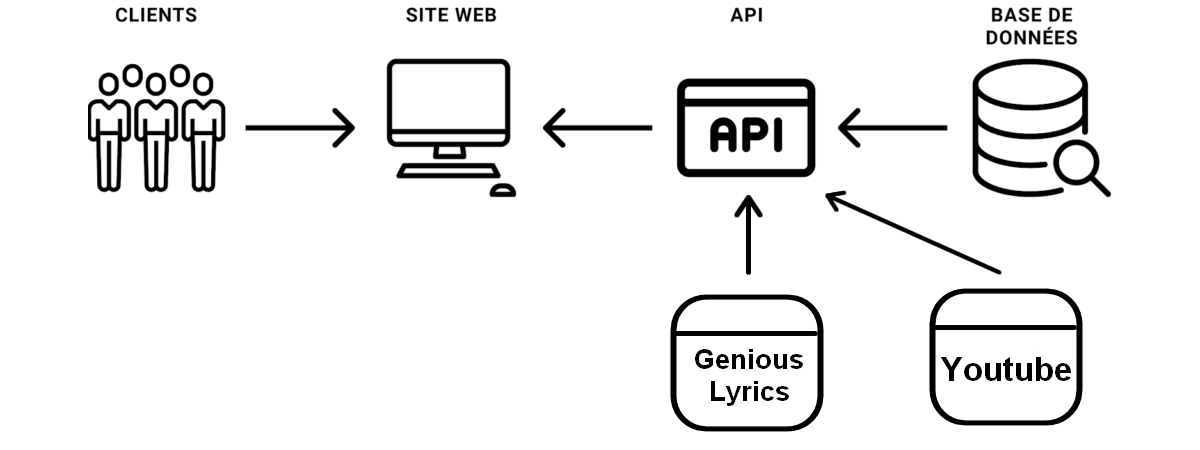
\includegraphics[scale=0.4]{fullstack.png}
	\caption{Organigramme de notre Application Fullstack}    
\end{figure}

\subsection{Principales fonctionnalités de notre site web}

Notre application a été réfléchie pour aider les utilisateurs à réviser les paroles de chansons qu'ils souhaitent apprendre, pour ce faire, nous proposons un grand nombre de fonctionnalités pour qu'ils s'améliorent tout en s'amusant.
\newline 

En visitant notre site web, les utilisateurs peuvent créer un compte ou se connecter s'ils en ont déjà un. Ils peuvent ensuite rechercher les chansons qu'ils souhaitent réviser en utilisant la barre de recherche intégrée.
\newline 

Une fois qu'ils ont trouvé une chanson, ils peuvent choisir la difficulté de la révision en fonction de leur niveau de compétence. Nous proposons également des exercices de type "trous à remplir" avec des réponses à trouver pour aider les utilisateurs à se souvenir des paroles.
\newline 

En plus de cela, les utilisateurs peuvent regarder des vidéos des chansons qu'ils ont recherchées, avec les paroles affichées en format karaoké pour un apprentissage plus facile. Ils peuvent également créer des dossiers pour organiser leurs chansons et faire des playlists personnalisées.
\newline 

Pour une expérience plus personnalisée, nous avons également inclus la possibilité d'enre- gistrer des chansons dans un dossier personnel, qui peut être géré directement depuis l'interface utilisateur.
\newline 

En résumé, notre application offre une plateforme complète pour aider les utilisateurs à réviser les paroles de leurs chansons préférées, en leur offrant des fonctionnalités utiles pour améliorer leur expérience d'apprentissage.

\newpage

\vspace*{1cm}

\subsection{Analyse des problèmes}


La conception d'une application pour aider les utilisateurs à réviser les paroles de leurs chansons préférées peut être un défi en soi, car il existe de nombreux problèmes potentiels qui peuvent survenir tout au long du processus.
\newline

L'un des problèmes les plus courants est la qualité des données. Il peut être difficile de trouver des sources de données fiables pour les paroles de chansons, et il peut y avoir des erreurs dans les paroles proposées par ces sources. Cela peut entraîner des difficultés pour les utilisateurs lorsqu'ils essaient de réviser les paroles de leurs chansons préférées.
\newline

Un autre problème courant est la gestion de la sécurité des données des utilisateurs. L'application doit s'assurer que les données personnelles des utilisateurs sont correctement protégées contre les attaques potentielles. Cela peut inclure des mesures telles que la cryptage des mots de passe et la gestion des accès utilisateurs.
En outre, l'application doit être facile à utiliser et intuitive pour les utilisateurs. Il est important de concevoir une interface utilisateur conviviale pour assurer une expérience utilisateur optimale. Les utilisateurs doivent être en mesure de trouver facilement les chansons qu'ils recherchent et d'utiliser les fonctionnalités proposées.
\newline
Enfin, l'application doit être adaptée à une grande variété d'appareils et de navigateurs différents. Les utilisateurs peuvent utiliser une variété de périphériques pour accéder à l'application, tels que des ordinateurs de bureau, des tablettes ou des smartphones, et l'application doit être capable de fonctionner sur tous ces appareils.
\newline

En somme, la conception d'une application pour aider les utilisateurs à réviser les paroles de leurs chansons préférées nécessite une attention particulière à la qualité des données, la sécurité, l'utilisabilité et la compatibilité multi-plateforme.
\newline
\newline

Une fois toutes ces problématiques étudiées et anticipées, nous nous sommes mis à la confection du diagramme de Gantt prévisionnel de notre projet.



\begin{figure}[H]
	\centering
	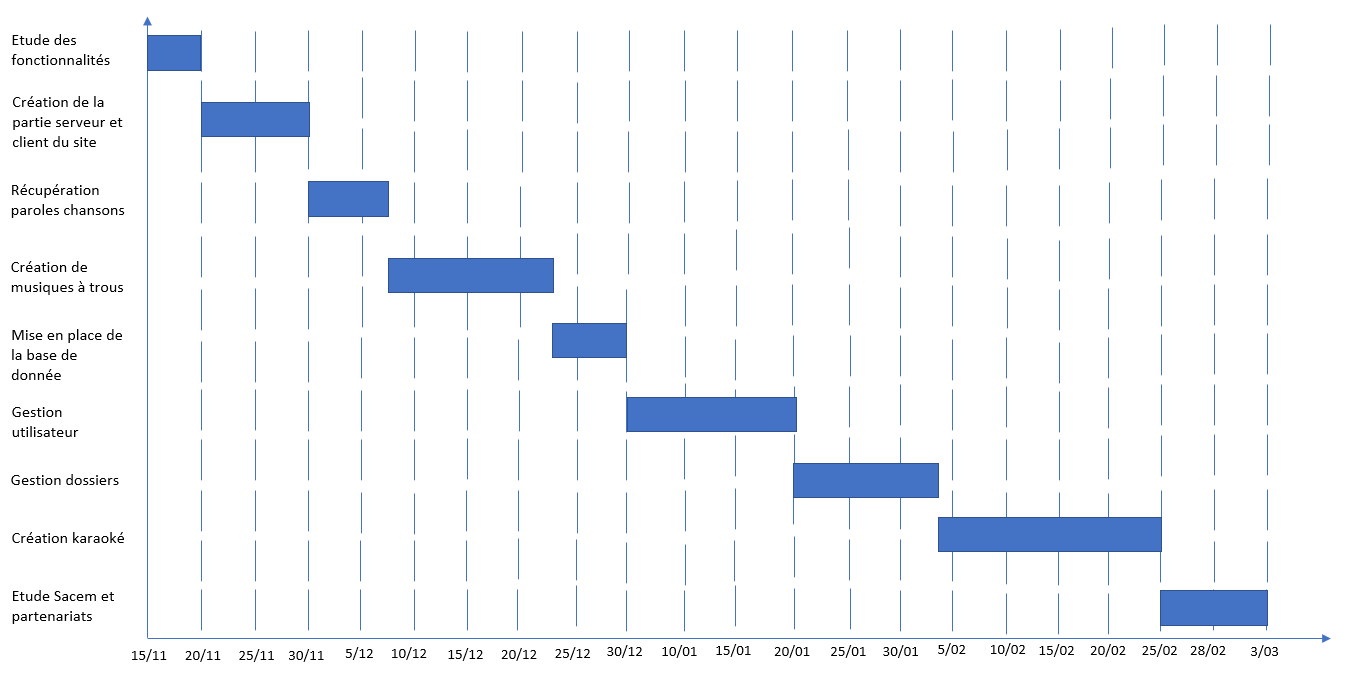
\includegraphics[scale=0.5]{ganttprevi.png}
	\caption{Diagramme de Gantt prévisionnel}    
\end{figure}

\section{Réalisation et conception}

\subsection{Nos choix}

\subsubsection{Le Back de notre site}

Pour la partie \gls{Back} de notre projet, nous avons choisi de prendre Node.js avec le module "Express".

\medskip

L'un de nous avait déjà travaillé sur cette technologie, donc cela permettait pour l'un, de ne pas partir de zéro et d'améliorer ses connaissances, et pour l'autre de découvrir une nouvelle technologie possiblement très utile pour notre filière de développement à l'ISIMA.

\medskip

De plus, Node.js est une technologie plus récente que d'autres langages qui peuvent gérer le côté serveur (comme PHP, par exemple). Ainsi, le module Express que nous utilisons est toujours maintenu à jour.

\medskip

Avec Express, nous pouvons en quelques minutes implémenter une \gls{API} assez facilement et parfaitement fonctionnelle. Cela nous a permis de bien scinder la partie \gls{Front} et \gls{Back} de notre projet.
Nous pouvons par exemple citer le langage PHP, où la partie serveur et la partie cliente sont parfois mélangées dans les mêmes fichiers.

Ici, nous avons le \gls{Back} dans un dossier et le \gls{Front} dans un autre, et ces deux aspects sont parfaitement indépendants ! On peut, par exemple, lancer le \gls{Back} pour faire des tests dessus sans toucher au \gls{Front}.

La partie \gls{Front} va pouvoir communiquer avec la partie \gls{Back} à l'aide de requêtes envoyées à celui-ci, auxquelles il va répondre.

\bigskip

Au niveau de l'organisation de notre \gls{Back}, nous avons séparé celui-ci en différentes couches.

\medskip

\begin{itemize}
	\item \textbf{"Controller Layer"} : réceptionne les requêtes et appelle les fonctions nécessaires en fonction de la demande. Elle répond ensuite aux requêtes. Elle correspond au fichier \textit{listen.js}.
	\item \textbf{"Business Layer"}: effectue tous les calculs de notre \gls{API}, on implémente dans celle-ci toutes les fonctions nécessaires au bon fonctionnement de l'\gls{API} (communication avec d'autres \gls{API}, création de trous à compléter dans les paroles etc...). Elle correspond à tous les fichiers \textit{gestion\_*.js} sauf "\textit{gestion\_database.js}"
	\item \textbf{"DataBase Layer"}: effectue toutes les requêtes à la base de donnée et renvoie les données récupérées. Elle est appelées par la couche business. Elle correspond au fichier \textit{gestion\_database.js}.
	
\end{itemize}

\bigskip

\begin{figure}[H]
	\centering
	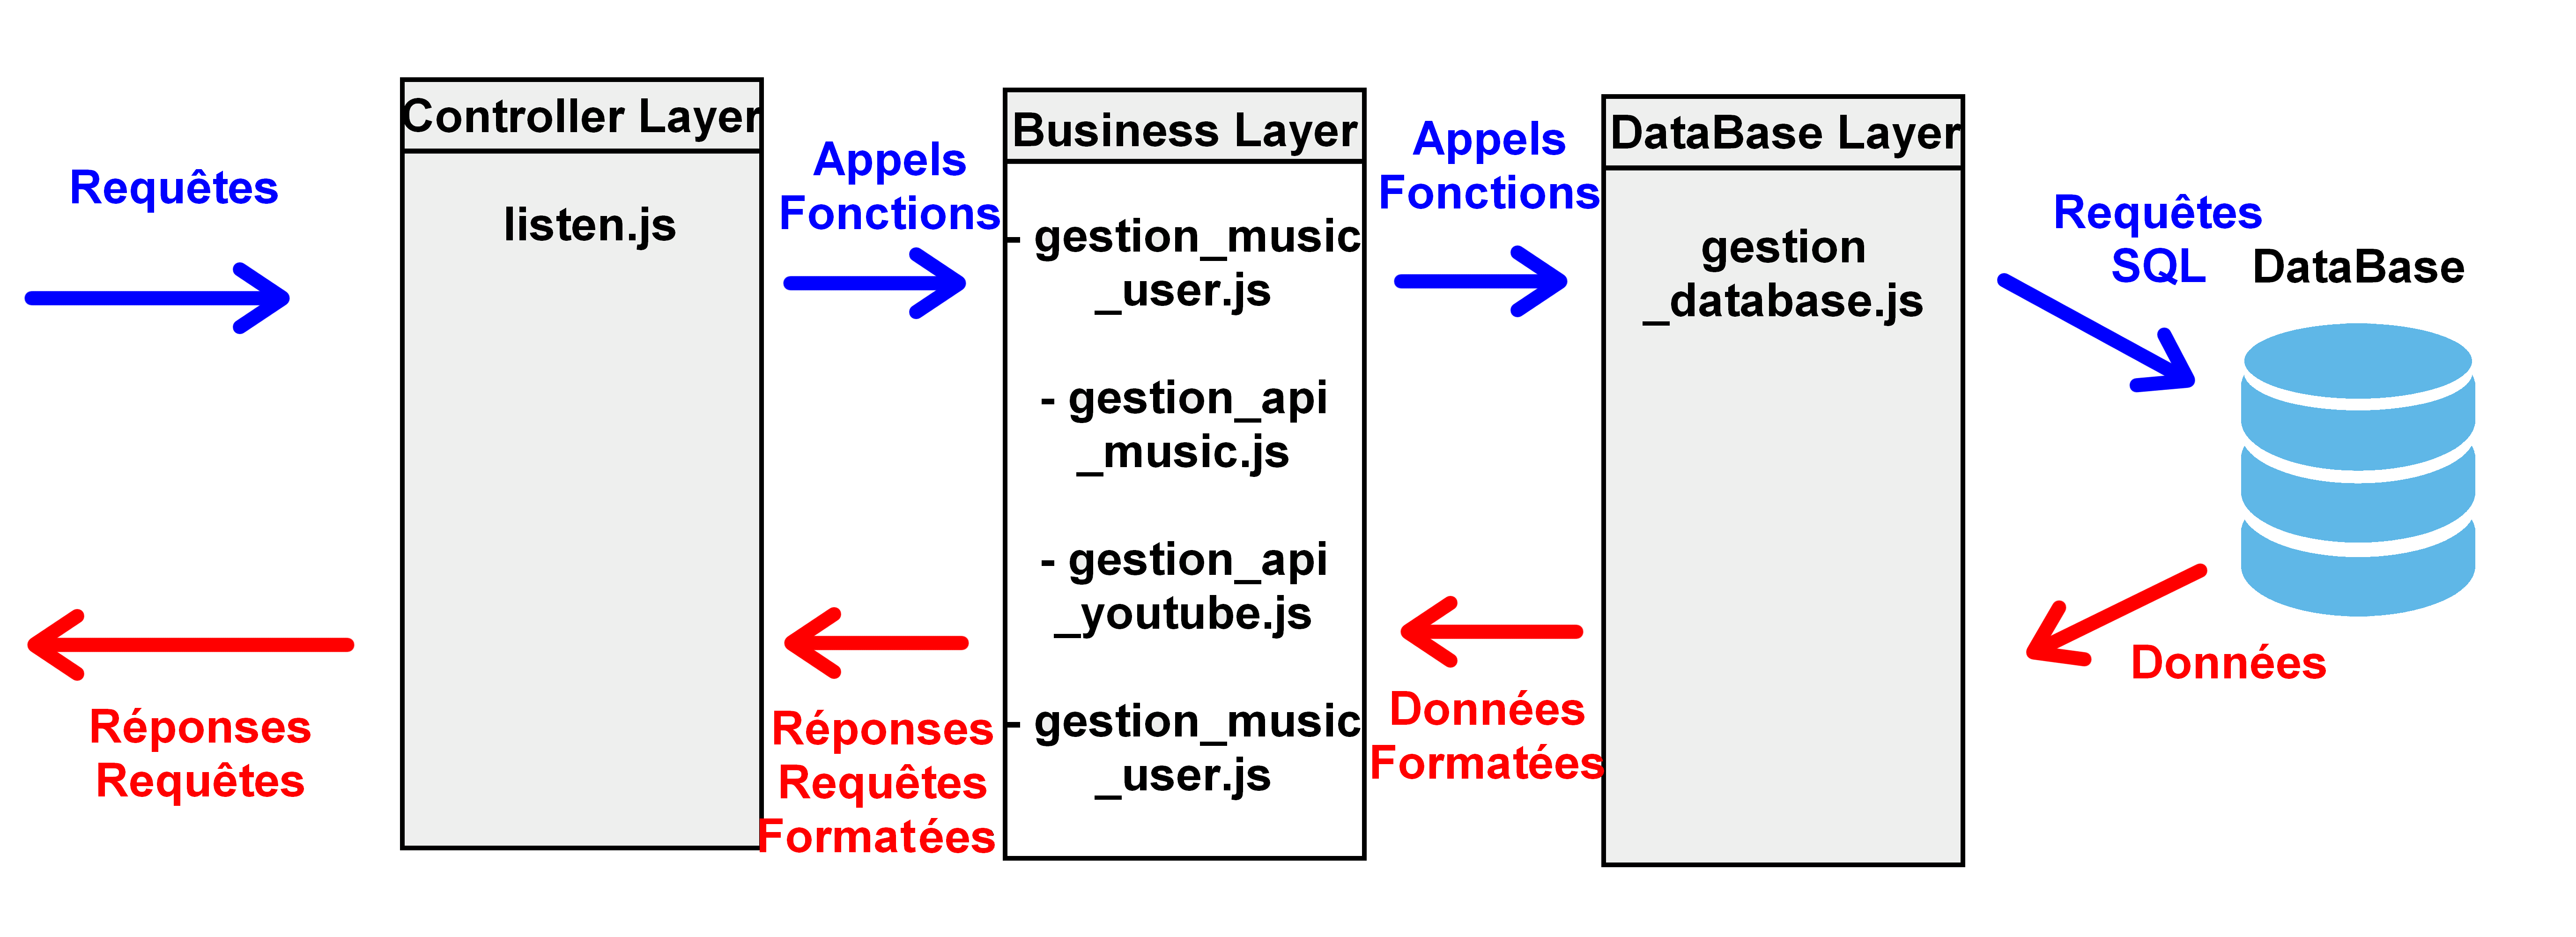
\includegraphics[scale=0.1]{api_couche.png}
	\caption{
	L'organisation de l'API}    
\end{figure}

\bigskip

Pour démarrer notre \gls{API}, nous lançons le fichier \textbf{server.js} qui positionne notre \gls{API} sur le port souhaité de notre machine. Ensuite, il se connecte à la base de données. Enfin, une fois que tout cela est effectué, nous activons les différents contrôleurs de l'\gls{API} et nous sommes prêts à recevoir des requêtes !

\begin{figure}[H]
	\centering
	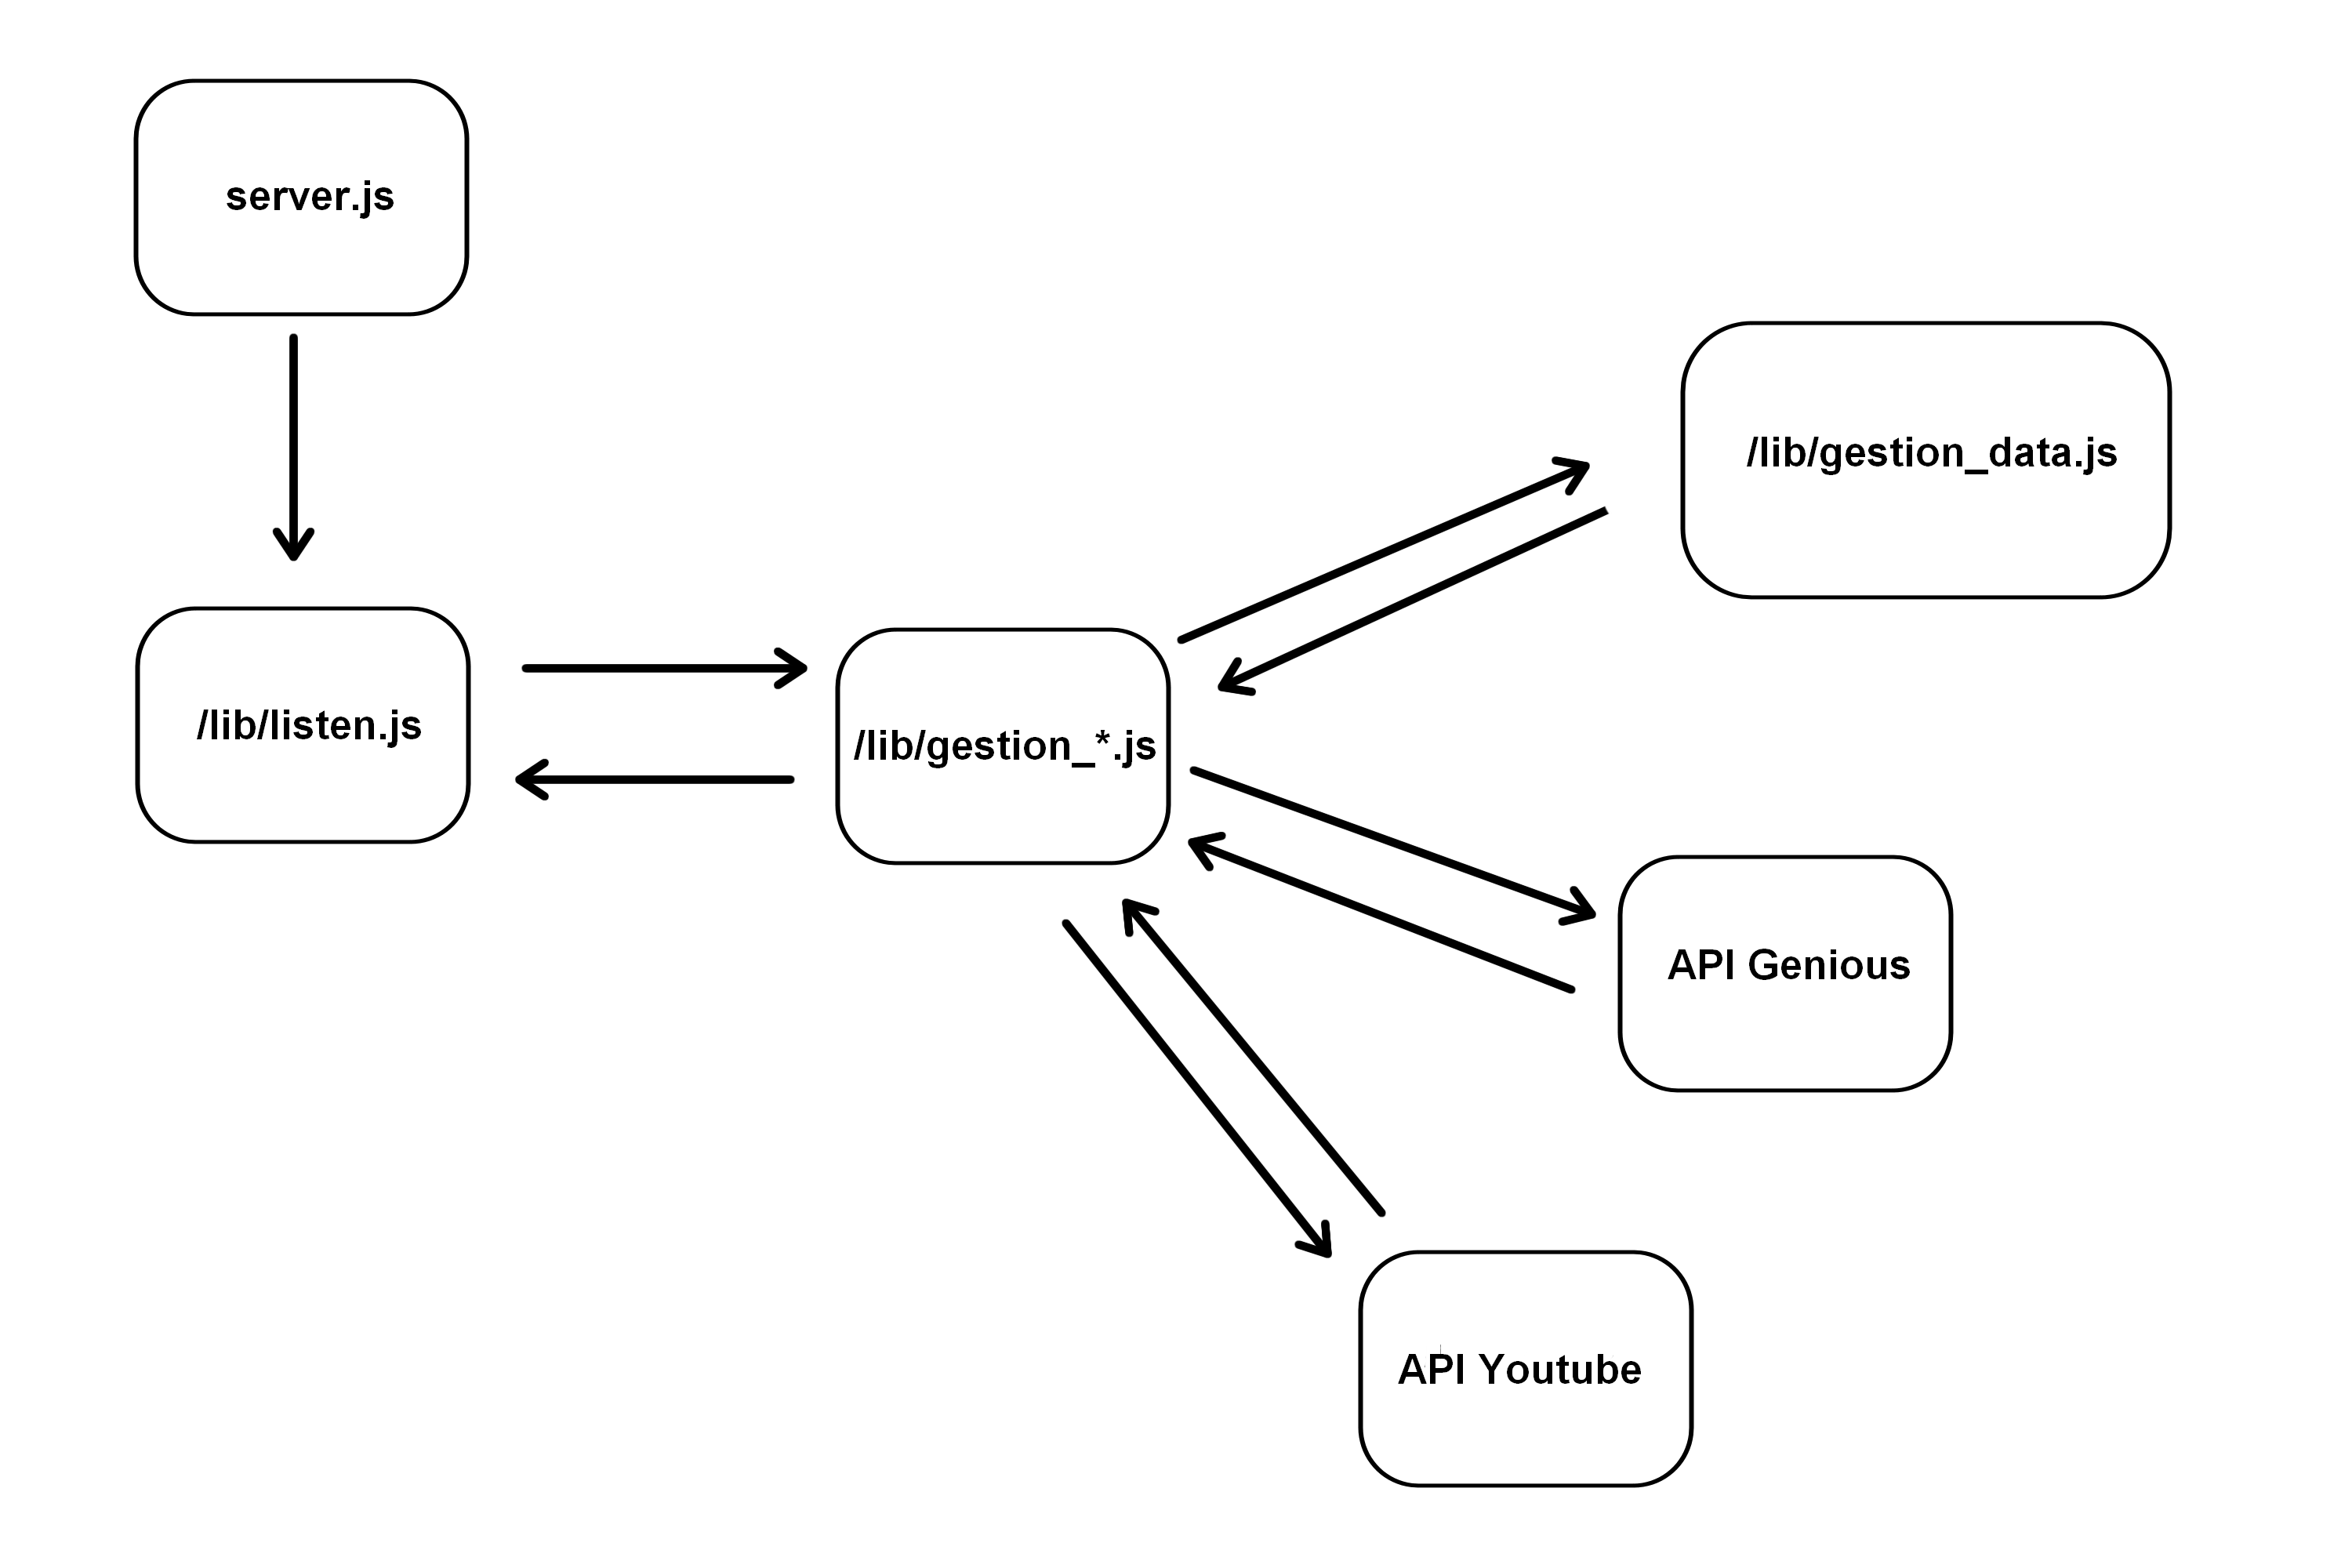
\includegraphics[scale=0.16]{api.png}
	\caption{Architecture de l'API}
\end{figure}

\medskip

On peut voir ici que nous communiquons avec d'autres \gls{API} publiques ! Nous vous expliquerons cela plus en détail par la suite.

\subsubsection{Le Front}

Pour la partie \gls{Front}, nous avons choisi d'utiliser un \gls{Framework} car ces technologies sont plus évoluées pour effectuer des comportements complexes.

\medskip

L'un des gros avantages de ces technologies est de pouvoir séparer notre application en plusieurs composants que nous allons pouvoir faire interagir les uns avec les autres ou encore inclure les uns dans les autres ! Cela permet de structurer plus proprement et efficacement une application.

\medskip

De plus, les \gls{Framework} sont des outils très puissants avec de nombreuses fonctionnalités pré-implémentées. Cela nous permet de ne pas avoir besoin de réinventer la roue et de nous concentrer sur nos propres implémentations.

\medskip

Ainsi, nous avons hésité entre le \gls{Framework} Angular et ReactJS qui sont les plus courants et les plus utilisés de nos jours. Notre choix s'est finalement porté sur Angular car nous étions familiers avec ce \gls{Framework} grâce à des projets personnels. 

\medskip

L'avantage de ce \gls{Framework} est qu'il utilise nativement \gls{Typescript} dans la version que nous utilisons, ce qui permet de créer des applications plus claires en typant les variables et les objets utilisés. De plus, chaque composant généré est composé d'un fichier \gls{HTML}, un fichier \gls{SCSS} et un fichier \gls{Typescript}, ce qui permet de bien séparer les trois aspects importants du \gls{Front} qui sont respectivement, dans l'ordre, le corps d'une page, son style et son comportement.

\bigskip

En plus d'Angular, nous avons utilisé le \gls{Framework} \textbf{Bootstrap} pour avoir des éléments graphiques au goût du jour. Par exemple, notre barre de navigation a été stylisée grâce à ce \gls{Framework}.

De plus, nous avons utilisé \textbf{PrimeNg} qui est une bibliothèque de composants Angular. Nous y retrouvons beaucoup d'éléments déjà créés très pratiques comme des dossiers (que nous avons utilisés pour la partie utilisateur) ou encore des boutons déjà stylisés.

\subsubsection{La base de donnée}

Pour la gestion de la base de données, plusieurs choix s'offraient à nous, mais nous avons décidé d'utiliser deux outils que nous connaissions bien : SQLPlus et MySQL Workbench. Ces outils ont été importants pour notre projet car ils nous ont permis de gérer efficacement la base de données, un élément essentiel de notre application qui stocke toutes les informations relatives aux chansons, aux utilisateurs et aux dossiers de playlists.
\newline

SQLPlus est un outil puissant pour gérer une base de données Oracle. Il nous a permis de créer et de gérer des \gls{table}s dans la base de données et de manipuler les données stockées. En utilisant cet outil, qui nous était familier, nous avons pu optimiser et automatiser un certain nombre de requêtes \gls{SQL}, nous faisant ainsi gagner du temps.
\newline

MySQL Workbench est lui un logiciel \gls{Open-source} permettant de gérer efficacement notre base de données. Cette application nous a permis de créer et de gérer des \gls{table}s dans la base de données, d'avoir accès aux données stockées et de manipuler ces même données à l'aide une interface utilisateur intuitive.
\newline
En utilisant ces deux outils, nous avons pu travailler efficacement sur la base de données de notre application, ce qui nous a fait gagner un temps précieux. Nous avons pu créer des \gls{table}s efficacement, gérer les contraintes, les index, et réaliser des requêtes complexes pour récupérer les données dont nous avions besoin. En outre, nous avons pu contrôler l'accès aux données ainsi que leur confidentialité grâce à ces outils.

Une fois ces deux outils choisis et configurés, nous devions alors sélectionner les différentes \gls{table}s que nous aurons à utiliser dans notre base de données. Le principal élément de notre application étant la gestion de dossiers dans lesquels un utilisateur peut enregistrer de la musique, nous avions déjà trois \gls{table}s qui nous semblaient assez logiques. La première est la base "Utilisateur" dans laquelle nous retrouverons le nom d'utilisateur, un ID utilisateur ainsi que son mot de passe. La seconde est la \gls{table} "Dossier" qui possède un numéro de dossier unique et qui est liée à un numéro d'utilisateur par une \gls{cle} secondaire. La troisième est la \gls{table} "Musique" car nous souhaitions garder une trace de chaque musique recherchée pour y avoir accès rapidement lors de la connexion à l'\gls{API}. Nous sauvegarderons donc un ID de la musique unique pour la différencier des autres, puis le nom de la musique ainsi que son chanteur. Enfin, une fois ces trois \gls{table}s créées, nous avons pensé à la création d'une \gls{table} que nous appellerons "MusiqueDansDossier" pour faire le lien entre la \gls{table} dossier et la \gls{table} musique sans supprimer les musiques de notre base à la suppression d'un dossier. Cette réflexion nous donne donc ces deux schémas pour bien comprendre notre conception de la base.

\begin{figure}[H]
	\centering
	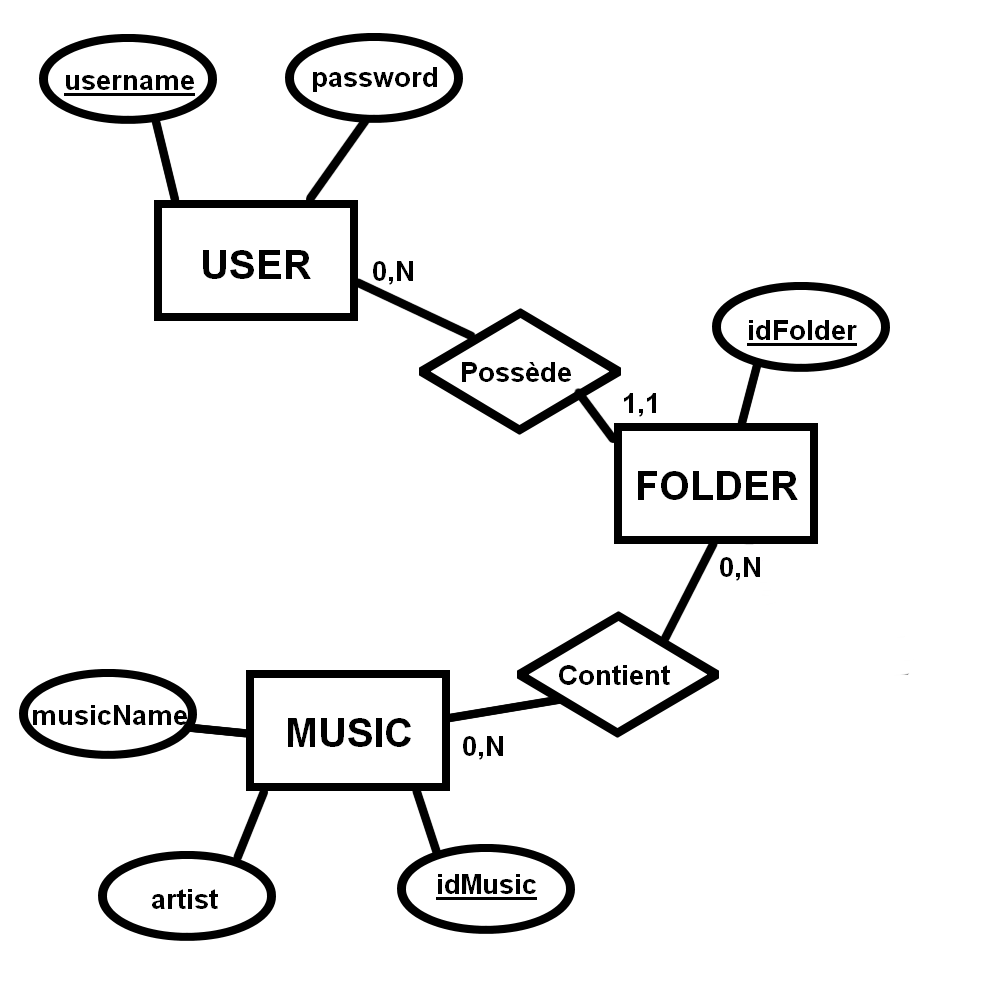
\includegraphics[scale=0.3]{diag_database.png}
	\caption{MLD de notre base de donnée}    
\end{figure}

\begin{figure}[H]
	\centering
	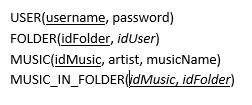
\includegraphics[scale=1]{table.png}
	\caption{Modèle relationnel de notre base de donnée}    
\end{figure}


\subsubsection{Choix des APIs}

Nous avons dû utiliser pour ce projet deux \gls{API}s publiques de deux entreprises différentes.

\medskip

Ces \gls{API}s nous permettent de récupérer des informations, comme par exemple des paroles de musique, et nous ont été très utiles. Pour chacune d'elles, nous avons dû nous inscrire sur le site de la documentation afin d'obtenir un \gls{token} pour communiquer avec elles.

\paragraph{Gestion des lecteurs vidéos avec paroles de musique \\\\}

La première est l'\gls{API} de \textbf{Youtube} de l'entreprise \textbf{Google}. Nous lui demandons, via une requête, le meilleur résultat pour une recherche avec les mots clés "\textit{nom musique}" + "\textit{nom artiste}" + "lyrics".

L'\gls{API} nous répond en envoyant une liste des 5 vidéos sur sa plateforme qui correspondent le mieux à la recherche et nous renvoyons le résultat numéro 1 à la partie utilisateur afin d'afficher le bon URL dans le lecteur.

\paragraph{Récupération des paroles de musique \\\\}

Notre second objectif était de trouver une \gls{API} qui pourrait nous fournir les paroles de musique et qui couvre donc un très grand nombre d'entre elles.

\medskip

Nous nous sommes tout d'abord penchés sur l'\gls{API} \textbf{ChartLyrics}, puis nous nous sommes rendus compte que celle-ci était trop incomplète. L'\gls{API} étant américaine, nous avions très peu de musique française dessus, ce qui est très dommage au vu de notre projet.

\medskip

Ainsi, nous nous sommes ensuite penchés sur une autre \gls{API} d'un site très connu qui couvre de très nombreuses musiques très diversifiées : \textbf{Genius Lyrics}.

Le problème de cette \gls{API} est que, dû à des problèmes de droits sur les paroles de musique (gérés en France par la \gls{SACEM}), nous ne pouvons pas obtenir les paroles de musique directement via des requêtes.

La solution est la suivante : l'\gls{API} nous fournit le lien vers la page web du site \textbf{Genius Lyrics}. Nous récupérons ce lien et, grâce au \gls{Web scraping}, nous arrivons à récupérer les paroles.

Dans l'ordre, la méthode pour récupérer les paroles d'une musique est donc la suivante :

\medskip

\begin{itemize}
	\item On contacte l'\gls{API} Genius Lyrics et on lui demande l'URL de la page du site qui contient les paroles.
	\item On aspire ensuite tout le code \gls{HTML} de la page web du site.
	\item Les paroles étant toujours dans la même balise \gls{HTML}, on les récupère tout en ignorant le reste du contenu de la page.
	\item Enfin, on formate les paroles pour qu'elles soient plus adaptées à de l'apprentissage.
\end{itemize}

\medskip

  \subsubsection{Chartes graphiques}

Pour ce qui est des choix visuels de notre plateforme web, la charte graphique finale se trouvant actuellement sur notre application a été choisie en dernier lors de notre conception. L'important pour nous étant que les fonctionnalités soient efficaces et permettent une utilisation satisfaisante du site. Nous avons tout de même fini par embellir ce projet à l'aide de plusieurs ressources disponibles en ligne. La première est Bootstrap, ce \gls{Framework} \gls{HTML} et \gls{CSS} préconstruit nous a permis de créer tout ce qui est menu déroulant ou animation comme sur la page d'accueil.
\newline

Pour la gestion des dossiers, nous avons utilisé des templates pour la création Angular disponibles sur PrimeNG, ce qui nous a permis de donner un style épuré à notre site mais aussi une utilisation agréable visuellement.

\subsection{Description détaillée} 

Pour cette description détaillée des fonctionnalités de notre site web, nous allons prendre l'ordre d'apparition de ces mêmes fonctionnalités lors de l'utilisation de notre site et non l'ordre de conception lors de notre projet.
\subsubsection{Gestion des comptes}

\paragraph{Création de compte \\\\}

La première fonctionnalité lors de l'arrivée sur notre site est celle de la création de compte. Pour pouvoir créer un compte, l'utilisateur doit renseigner son nom d'utilisateur ainsi que son mot de passe qu'il doit par la suite confirmer. Une fois toutes ces informations récoltées, deux phases de vérifications s'opèrent. La première est plutôt simple et vérifie juste que les deux mots de passe renseignés soient bien les mêmes. Ensuite, la deuxième vérification se trouve en aval de l'insertion en base de données. Ici, on vérifie par une requête dans notre \gls{table} utilisateur qu'il n'existe aucun nom d'utilisateur identique à celui à insérer. Une fois ces vérifications passées, nous insérons dans notre \gls{table} utilisateur une ligne avec le nom d'utilisateur renseigné et avec un mot de passe préalablement \gls{sale} puis \gls{chiffre}. Une fois l'insertion effectuée, nous sommes redirigés sur une page de connexion.


\paragraph{Connexion au site web \\\\}

Lorsque nous possédons un compte, nous devons maintenant nous connecter. L'utilisateur doit renseigner son nom d'utilisateur et son mot de passe pour pouvoir vérifier la concordance des mots de passe et lui accorder une connexion. Si, après notre requête en base de données, le mot de passe renseigné et celui en base de données sont identiques, alors l'utilisateur se connecte sur le site avec son compte, ce qui va lui permettre d'effectuer un certain nombre de fonctionnalités impossibles sans connexion, comme nous allons le voir plus bas dans la gestion des dossiers. Lors de la connexion de ce même utilisateur, nous lui créons un \gls{token} afin de vérifier les permissions d'accès à la base de données lors d'insertions ou de suppressions. Ce \gls{token} nous permet également de faire une requête en base pour récupérer les dossiers que possède l'utilisateur pour lui afficher sur son menu personnalisé.

\subsubsection{Gestion des paroles}

Le principe de notre site étant de donner la possibilité à un utilisateur de réviser ou apprendre les paroles des musiques qu'il désire, une grande partie de nos fonctionnalités se trouve dans cette gestion des paroles. 

\paragraph{Recherches de musiques \\\\}

Chronologiquement, la première fonctionnalité que nous avons développée est cette re- cherche de musiques et donc de paroles. L'utilisateur peut donc choisir le nom de la musique recherchée ainsi que le nom du chanteur. Une fois ces deux informations récupérées, on met alors en place une longue suite d'algorithmes pour permettre d'afficher les paroles recherchées. Pour commencer, nous utilisons les informations de recherche de l'utilisateur pour former manuellement une requête composée et l'envoyer à l'\gls{API} Genius Lyrics. Une fois cette requête effectuée et notre accès à l'\gls{API} confirmé, nous récupérons les paroles que nous fournit l'\gls{API} grâce au \gls{Web scraping} que nous avons présenté ci-dessus. Grâce à cette récupération de code, nous pouvons renvoyer l'intégralité des paroles à notre site web et les afficher comme bon nous semble.

\paragraph{Création des musiques à trous \\\\}

Une fois ces paroles récupérées et formatées à notre convenance, nous les avons modifiées afin de permettre à l'utilisateur de posséder de nombreux outils pour apprendre ces paroles. L'outil principal de cette fonctionnalité est le remplissage de texte à trous afin de s'entraîner à connaître les mots manquants. Pour la création de ces mots manquants, le principe est plutôt simple. Nous utilisons une fonction aléatoire afin de supprimer certains mots au milieu des paroles de la chanson. Nous avons fait le choix de parsemer les mots manquants et non d'enlever des phrases pour permettre de travailler toutes les parties de ces mêmes chansons. Une fois un mot sélectionné comme manquant par notre algorithme, nous affichons une case permettant à l'utilisateur de saisir le mot de son choix. Le site web donne le choix à l'utilisateur de choisir la difficulté qu'il souhaite pour l'apprentissage de nos musiques.
\newline

- La difficulté 1 affiche purement et simplement les paroles sans trou afin de pouvoir les lire plus facilement. 

- La difficulté 2 affiche cette fois-ci un nombre de mots manquants à hauteur de 15\%, et indique à l'utilisateur le nombre de lettres que possède chaque mot manquant.

- La difficulté 3 est sensiblement la même que la difficulté 2, mais augmente le pourcentage de mots manquants à 30\%.

- Enfin, la difficulté 4 possède la même fréquence de mots manquants que la difficulté 3, mais n'affiche cette fois-ci plus le nombre de lettres dans le mot manquant, ce qui augmente drastiquement la difficulté de remplissage.  
     
\paragraph{Vérification des réponses manquantes \\\\}

Pour les difficultés de 2 à 4, il nous fallait donc un système de vérification de réponse entre les mots manquants et les mots saisis par l'utilisateur. Pour ce faire, il n'y a rien de plus simple. Lorsque nous choisissons un mot comme manquant dans notre affichage de révision, nous l'insérons aussi dans un tableau de mots manquants pour avoir accès à tous les mots lors de la vérification. Une fois ces mots enregistrés, nous faisons simplement une comparaison de chaîne de caractère entre le mot enregistré dans notre tableau de mots et celui saisi lors de l'entraînement. Si les mots concordent, nous affichons la case en vert et nous enlevons la possibilité de remplir ce texte à nouveau. Si c'est faux, nous l'affichons en rouge et l'entraînement continue.

\paragraph{Utilisation du lecteur YouTube \\\\}

Une dernière fonctionnalité disponible dans notre mode d'entraînement n'a pas été évoquée jusqu'ici, il s'agit de l'incrustation vidéo de la musique recherchée en bas de page sous format karaoké. Pour obtenir cette vidéo, le principe est sensiblement le même que pour récupérer les paroles sur l'\gls{API} Genius Lyrics. Nous avons créé un \gls{token} nous donnant accès à l'\gls{API} YouTube et une fois ceci effectué, nous pouvons encore une fois créer une requête avec les informations de la musique recherchée pour directement afficher la première vidéo disponible sur YouTube en ajoutant l'information "karaoke". Ceci nous permet de pouvoir nous mettre en condition pour participer à l'émission "N'oubliez pas les paroles" en voyant les paroles défiler en même temps que la musique en fond.  

\subsubsection{Gestion des dossiers playlist}

Le principal avantage de pouvoir se connecter avec un compte utilisateur à un tel site web est d'avoir accès à des données enregistrées en base de données pour pouvoir les récupérer et pour pouvoir enregistrer des préférences utilisateur.

\paragraph{Ajout de dossiers \\\\}

La première étape si l'on veut pouvoir sauvegarder des musiques dans nos préférences est de créer un dossier affilié à notre nom utilisateur. Dans le menu personnalisé de l'utilisateur, on choisit le nom du dossier à créer, puis on l'ajoute à notre base de données. Pour l'ajouter à notre base de données, nous effectuons tout de même une vérification pour éviter les problèmes de vol de données ou d'intrusion dans notre base. Bien que ces données ne soient pas catégorisées comme sensibles, il est toujours bon de donner le moins de privilège possible à l'utilisateur afin d'être sur qu'il ne va pas profiter de certaines failles. C'est pourquoi nous avons créé un \gls{token} utilisateur précédemment lors de la création de compte. Lors de l'ajout ou de toute autre manipulation de nos données personnelles dans la base de données, le \gls{token} utilisateur est vérifié pour pouvoir identifier quel utilisateur effectue quelle modification sur quelles bases. Si les permissions sont accordées, alors nous créons un dossier affilié à un utilisateur dans notre base de données.

\paragraph{Ajout de musiques dans un dossier \\\\} 

Une fois ces dossiers créés, nous avons maintenant la possibilité d'enregistrer une musique de notre choix dans le dossier de notre choix. Encore une fois, la vérification du \gls{token} utilisateur est effectuée, mais à cela vient se rajouter une vérification pour éviter d'avoir des doublons dans notre base de données. Il nous semblait inutile de posséder deux fois la même version d'une musique dans un même dossier, c'est pourquoi cette vérification est faite avant de faire l'insertion dans la \gls{table} reliant les dossiers aux musiques. Du côté de la base de données, on stocke seulement les informations nécessaires à la recherche sur les différentes \gls{API}.

\paragraph{Suppression d'une musique \\\\}

Comme nous savons que les goûts des utilisateurs sont amenés à changer, nous avons aussi implémenté une fonction permettant de supprimer une musique d'un de nos dossiers personnels. Pour la suppression, il s'agit toujours du même procédé, nous vérifions toujours le \gls{token}, puis que la musique existe bien dans le dossier avant de la supprimer de la base de données.

\paragraph{Suppression de dossier \\\\}

Enfin, la dernière fonctionnalité majeure du site web n'est nulle autre que la suppression d'un dossier. Tout comme la suppression de musique, l'utilisateur peut modifier ses dossiers comme bon lui semble au cours du temps en supprimant de la base de données le dossier choisi ainsi que les musiques qu'il contenait. À noter que pour toutes les requêtes de base de données, une validation est demandée pour éviter de supprimer le mauvais dossier par mégarde.

\subsection{Le déroulement du projet}

Notre façon de travailler était comparable à une méthode agile de développement, c'est-à-dire que nous avons séparé le projet en différentes parties comme vous l'avez vu plus tôt (partie parole, partie utilisateur, etc.). À chaque partie du projet, nous avons effectué un \gls{sprint} durant lequel nous suivions toujours le même schéma de travail :

\begin{itemize}
	\item Nous avons implémenté ou modifié la base de données.
	\item Nous avons relié la partie serveur (\gls{Back}) du projet à la base de données.
	\item Nous avons implémenté les fonctionnalités nécessaires côté serveur.
	\item Nous avons relié la partie utilisateur (\gls{Front}) à la partie serveur (\gls{Back}).
	\item Nous avons testé la fonctionnalité implémentée.
\end{itemize}

\begin{figure}[H]
	\centering
	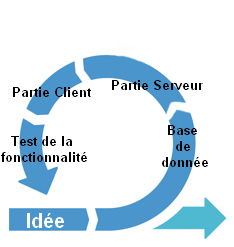
\includegraphics[scale=1]{agile.png}
	\caption{Les différentes étapes d'ajout d'une fonctionnalité}
\end{figure}

Finalement, nous avons effectué à la fin un embellissement de la partie utilisateur (\gls{Front}) car il est très important d'avoir une interface utilisateur très agréable d'utilisation pour faciliter l'interaction avec notre application.

Maintenant, voyons en détail ce que chaque partie d'un \gls{sprint} impliquait.

\subsubsection{Exemple complet d'un Sprint}

\paragraph{Modification de la base de données \\\\}

À chaque nouveau \gls{sprint}, nous regardions tout d'abord si une modification de la base de données était nécessaire.

Si c'était le cas, nous reconstruisions notre base de données en ajoutant les nouvelles \gls{table}s et \gls{colonne}s nécessaires.

Cela impliquait de modifier le script \textbf{setupDatabase.js} pour que nous ayons chacun de notre côté, en local, exactement la même base de données.

Lorsque cela était fait, nous effectuions chacun de notre côté des tests en local sur nos machines afin de vérifier que nos bases de données avaient le même comportement.

\paragraph{Mise en lien de la base de données avec notre partie serveur \\\\}

Ensuite, on reliait la base de données à la partie serveur.

\medskip

Le principe est le suivant : on créait des requêtes \gls{SQL} qui permettent de récupérer les données dont on a besoin pour les futures implémentations.

On incluait ensuite ces requêtes dans le code \gls{Javascript} de notre \gls{Back} dans le fichier \textit{gestion\_database.js}.

Enfin, on créait dans la "couche business" toutes les fonctions nécessaires pour formater les données comme il nous faut.

C'est durant cette partie aussi que l'on a créé les fonctions qui envoient des requêtes \gls{HTTP} à des \gls{API}s si nécessaire. Comme avec la base de données, après avoir reçu les données, on les formatait afin de mieux les exploiter dans le \gls{Front}.

\paragraph{Mise en lien de la partie serveur avec la partie utilisateur \\\\}


Au final, il ne nous restait plus qu'à créer côté client les nouveaux composants Angular nécessaires pour implémenter la nouvelle fonctionnalité. Ensuite, on avait juste à créer les requêtes à envoyer à notre partie serveur pour récupérer les éléments nécessaires côté client.

\subsubsection{Nos différents Sprints effectués}

Nous avons effectué ainsi 3 \gls{sprint}s durant le développement de notre application web.

\begin{itemize}
	\item Le développement de la partie entrainement avec les paroles
	\item Le développement de la partie inscription/connexion
	\item Le développement de la partie stockage des musiques avec les dossiers utilisateurs
\end{itemize}


\subsubsection{Embellissement du front}

Au départ, nous avons cherché à développer une application fonctionnelle sans nous pencher de trop sur l'apparence. Nous avons essayé de développer toutes les fonctionnalités que nous voulions ajouter en nous assurant que celles-ci ne présentaient aucun bug.

\medskip

Après nous être assurés que tout fonctionnait comme nous le souhaitions, nous avons décidé à la toute fin d'embellir le \gls{Front}. Nous avons pour cela utilisé nos connaissances en \gls{CSS} ainsi qu'en Bootstrap.

\medskip

Ayant quelques notions d'IHM (interface homme machine), nous savons que l'apparence d'un site web est une étape primordiale du développement logiciel. En effet, il ne faut pas utiliser, par exemple, des contrastes de couleur qui pourraient gêner certaines personnes comme les daltoniens.

De plus, chaque élément du site doit être intuitif et c'est ainsi que nous avons essayé de faire des fonctionnalités très simples d'utilisation (boutons simples, pas trop de détails, etc.).

\begin{figure}[H]
	\centering
	\begin{minipage}{.5\textwidth}
		\centering
		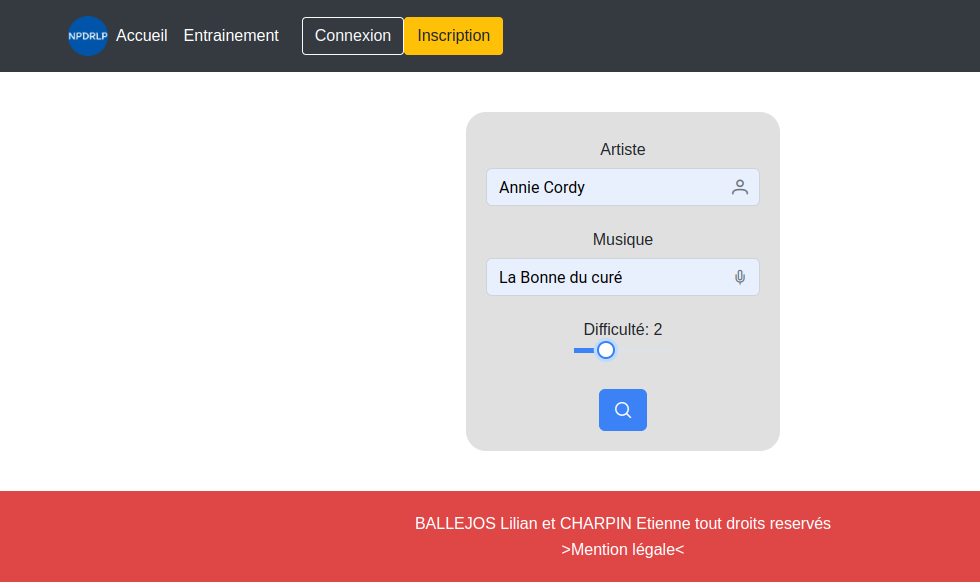
\includegraphics[scale=0.25]{avantfront.png}
	\end{minipage}%
	\begin{minipage}{.5\textwidth}
		\centering
		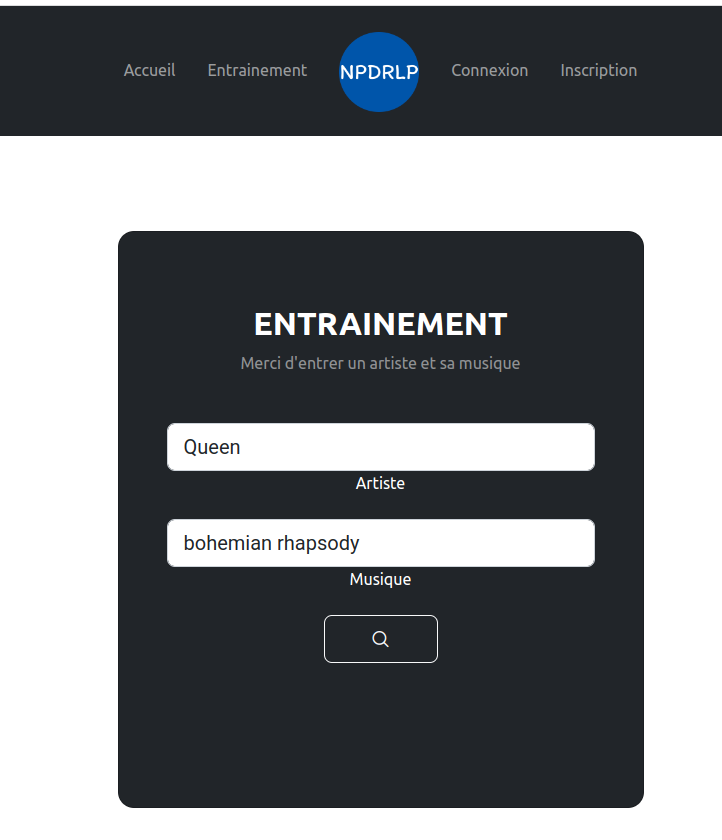
\includegraphics[scale=0.25]{apresfront.png}
	\end{minipage}
	\caption{Avant / Après de l'apparence de la partie client}
\end{figure}

\subsubsection{Le partage du travail} 

Lors de notre projet, le partage des tâches importantes s'est fait plutôt naturellement au sein de notre groupe. Lilian étant très familier avec l'utilisation de NodeJS et Etienne plutôt du côté base de données et \gls{Front}, nous avons agi de façon agile comme expliqué précédemment. En fonctionnant sur des mini-\gls{sprint}s pour implémenter nos fonctions une par une, Lilian codait la partie \gls{Back} permettant de faire le lien de l'application aux différentes \gls{API}. Etienne, lui, codait la partie algorithmique permettant aux fonctionnalités du site de fonctionner afin de pouvoir réviser les paroles ou bien de faire la gestion de base de données.
\newline


Cette méthode de travail a donc permis à Lilian de coder l'\gls{API} Genius Lyric afin qu'Etienne puisse formater les paroles pour les afficher dans le site et créer les différents niveaux de difficultés. Pour l'affichage YouTube, c'est Lilian qui s'est organisé pour créer le \gls{token} YouTube permettant de créer un lecteur vidéo affichant notre requête de façon correcte. Pendant ce temps, Etienne créait les fonctions permettant de créer la base de données ainsi que ses \gls{table}s, mais aussi les insertions, sélections et suppressions. Grâce à cela, Lilian a pu implémenter la vérification du \gls{token} utilisateur pour contrôler les requêtes. Il s'est aussi occupé de la gestion du chiffrement et du salage du mot de passe dans la base de données. Enfin, pour ce qui est de l'aspect visuel, c'est majoritairement Lilian qui a eu la charge de rendre le site visuellement agréable lors de nos dernières heures de travail.
\newline   

Bien que nous ayons prévu un planning anticipé de ce que nous allions faire grâce à notre diagramme de Gantt prévisionnel, nous nous sommes rendu compte au moment de notre diagramme de Gantt réel que certaines tâches avaient été supprimées et que les dates avaient évidemment bougé.

\begin{figure}[H]
	\centering
	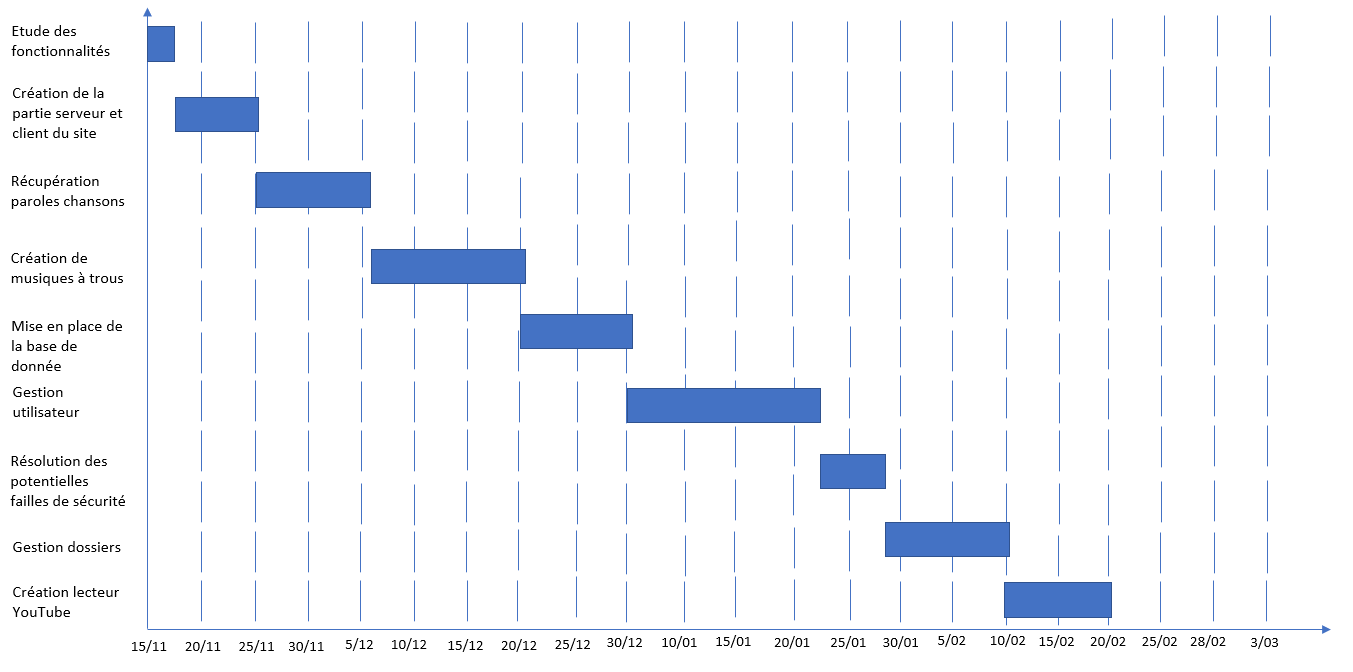
\includegraphics[scale=0.5]{ganttreel.png}
	\caption{Diagramme de Gantt réel}    
\end{figure}

\section{Résultats et discussions}

\subsection{Prise en Main de l'Application Web}

\subsubsection{Comment lancer l'Application Web}

Nous n'avons pas exporté notre projet car il est encore en phase de développement. Pour lancer notre application sur une machine, il faut suivre quelques étapes.

\newpage

\paragraph{Installation et configuration (à faire une fois) \\\\}

Tout d'abord, il vous faut installer quelques logiciels :

\begin{itemize}
	\item \textbf{mysql} : Pour la gestion de la base de données.
	\item \textbf{node} ainsi que son package manager \textbf{npm} : Pour lancer la partie serveur et la partie utilisateur.
\end{itemize}

\bigskip

Ensuite, vous pouvez trouver notre projet sur GitHub à ce lien :

\textbf{\href{https://github.com/LIlianHub/projetZZ2-NPDRLP}{https://github.com/LIlianHub/projetZZ2-NPDRLP}}

\bigskip

Après avoir installé le projet sur votre machine, il va falloir aller dans les dossiers "\textit{backend-api}", "\textit{frontend-angular}" et "\textit{setupDataBase}" et exécuter \textbf{dans ces 3 dossiers} la commande \textbf{npm i}, qui va permettre d'installer les dépendances nécessaires.

\bigskip

Une fois cela fait, lancez \textbf{mysql} et créez une nouvelle base de données nommée \textbf{npdrlp} en entrant la commande \textbf{CREATE DATABASE npdrlp}.

\bigskip

Ensuite, rendez-vous dans le dossier \textit{setupDataBase} et exécutez \textbf{node setup.js} afin de lancer la configuration de la base de données.

\paragraph{Lancer l'application \\\\}

Pour lancer l'application et la tester, il vous suffit de suivre ces deux étapes :

\begin{itemize}
	\item Dans \textit{backend-api}, entrez la commande \textbf{node server.js}.
	\item Dans \textit{frontend-angular}, entrez la commande \textbf{ng serve}.
\end{itemize}

Une fois cela fait, vous pouvez accéder à notre projet en local à cette adresse :

\textbf{\href{http://localhost:4200}{http://localhost:4200}}

\subsubsection{Arrivée sur le site}

La page d'accueil du site web est défilante et vous informe du concept de notre application, de qui nous sommes et de nombreuses autres informations.

Nous pouvons si nous le souhaitons changer le code source du site web afin de rajouter des éléments à l'accueil, cela sans difficulté !

\bigskip

En haut de la page, vous pouvez voir les différentes fonctionnalités de notre site web proposées dans le \gls{header}. Vous avez la possibilité d'aller à l'accueil (là où nous sommes actuellement) mais aussi dans la partie entraînement. Vous pouvez également vous inscrire ou, si cela est déjà fait, vous connecter !

Le \gls{header} va changer en fonction de si vous êtes connecté ou non. Si vous êtes connecté, au lieu de la possibilité de vous inscrire ou de vous connecter, vous aurez la possibilité d'aller à votre menu utilisateur ou de vous déconnecter.

\begin{figure}[H]
	\centering
	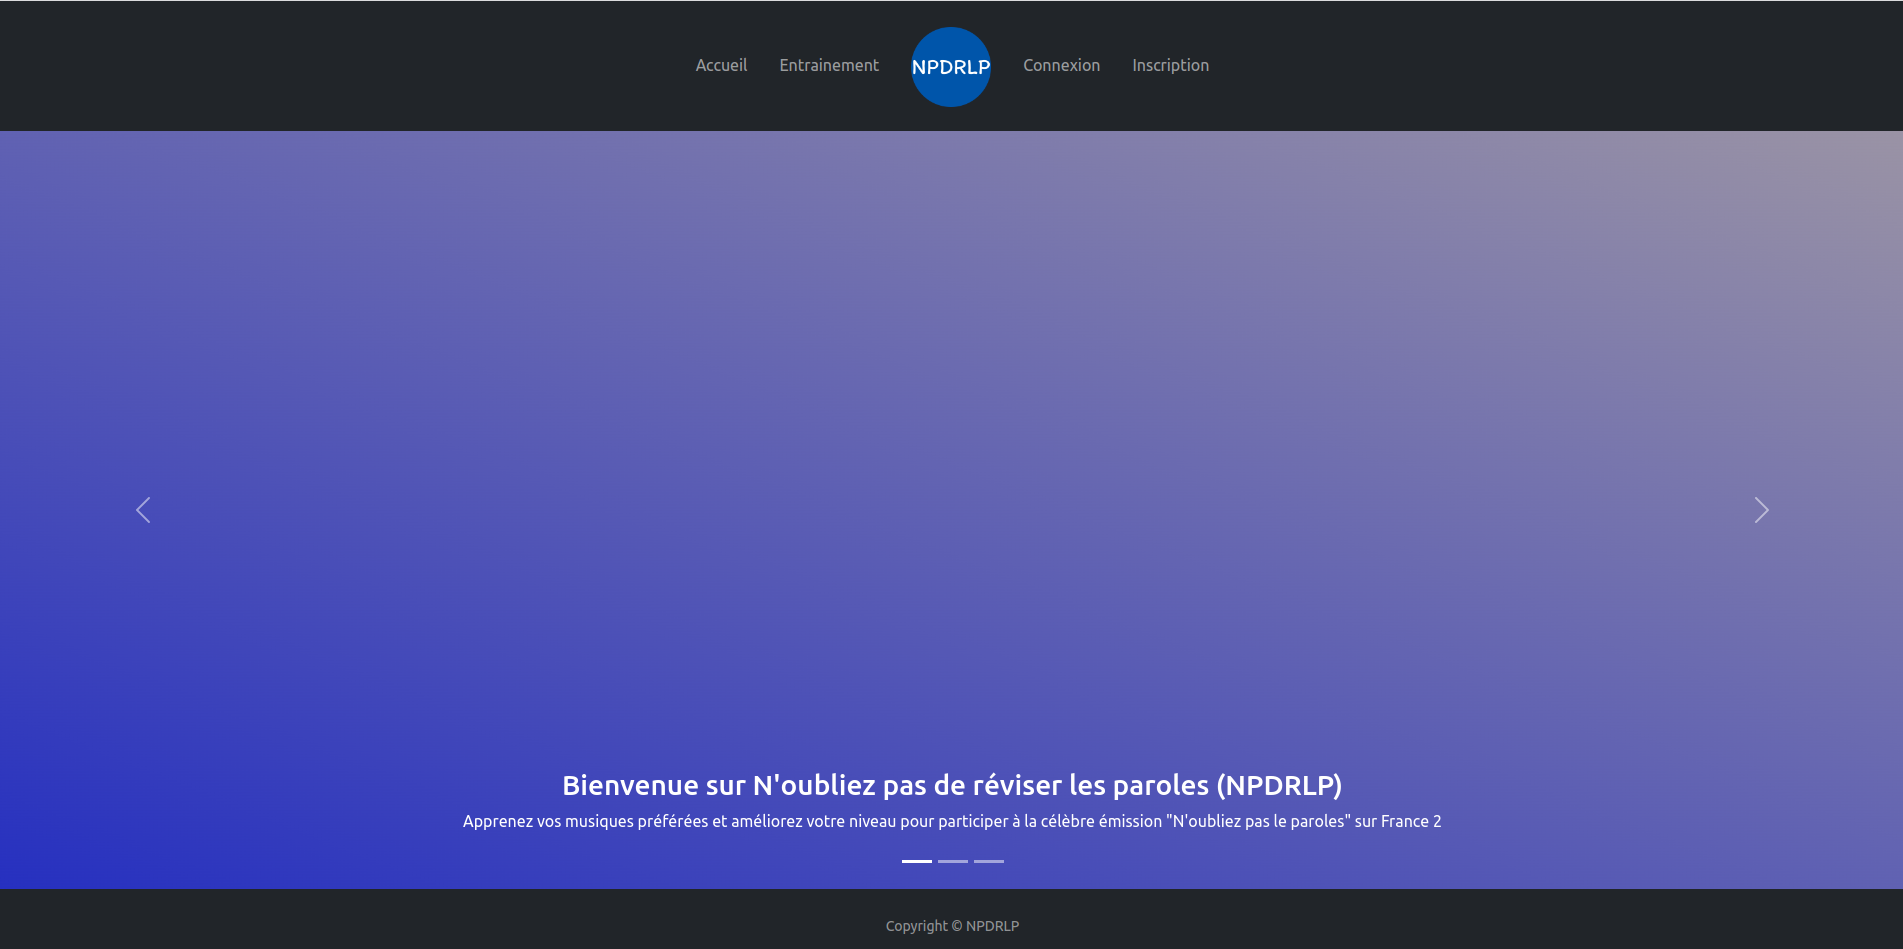
\includegraphics[scale=0.25]{accueil.png}
	\caption{La page d'accueil de notre site web.}
\end{figure}


\subsubsection{Partie Entrainement}

En arrivant dans la partie entraînement, un formulaire vous demande de renseigner à la fois le nom de l'artiste ainsi que la musique que vous souhaitez apprendre.

\begin{figure}[H]
	\centering
	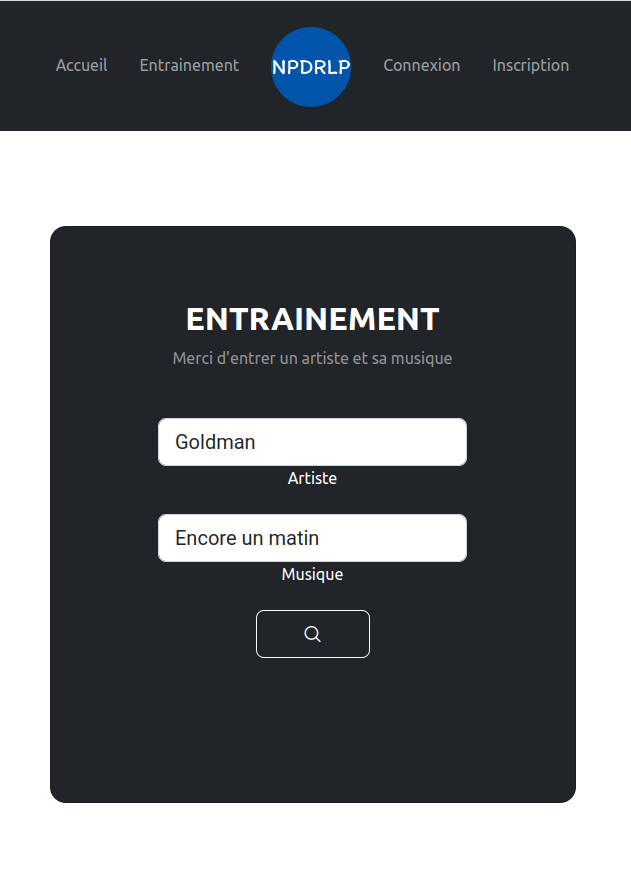
\includegraphics[scale=0.25]{rechercheparole.png}
	\caption{Formulaire de recherche de paroles}
\end{figure}

Si vous renseignez quelque chose de faux ou erroné, l'application affichera un message d'erreur vous informant que les paroles n'ont pas pu être trouvées.

Si les informations renseignées sont correctes, alors l'intégralité des paroles de la musique est affichée sur votre écran. En dessous de celles-ci, vous trouverez un lecteur YouTube avec une vidéo de la musique recherchée.

\begin{figure}[H]
	\centering
	\begin{minipage}{.5\textwidth}
		\centering
		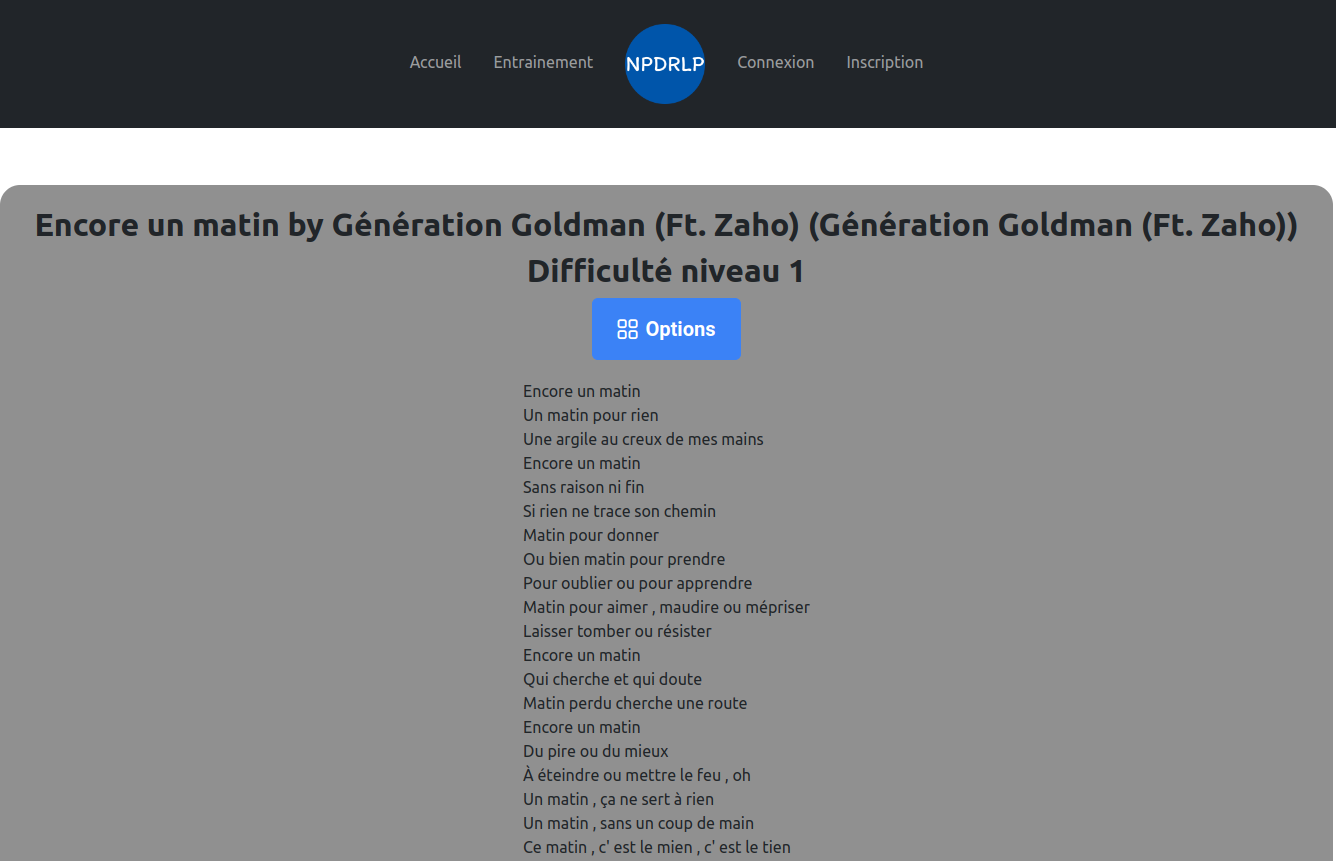
\includegraphics[scale=0.15]{parole.png}
	\end{minipage}%
	\begin{minipage}{.5\textwidth}
		\centering
		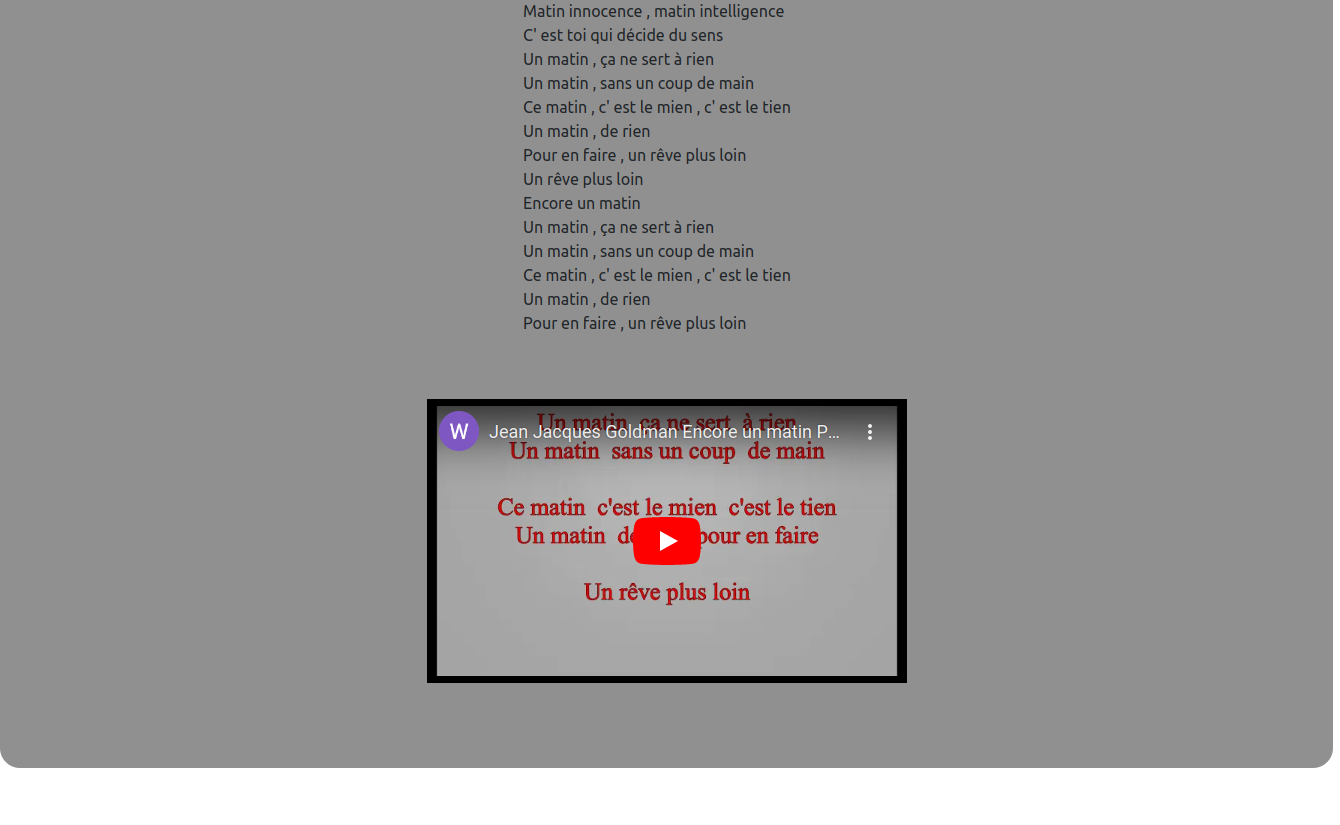
\includegraphics[scale=0.15]{ytbparole.png}
	\end{minipage}
	\caption{Affichage des paroles dans le mode entraînement}
\end{figure}

Enfin, nous trouvons au-dessus des paroles un bouton "Options" sur lequel nous pouvons cliquer. Lors du clic sur celui-ci, un menu apparaît sur la gauche avec deux fonctionnalités :

\begin{itemize}
	\item Sauvegarder la musique dans un dossier
	\item Changer la difficulté
\end{itemize}

\bigskip

\begin{figure}[H]
	\centering
	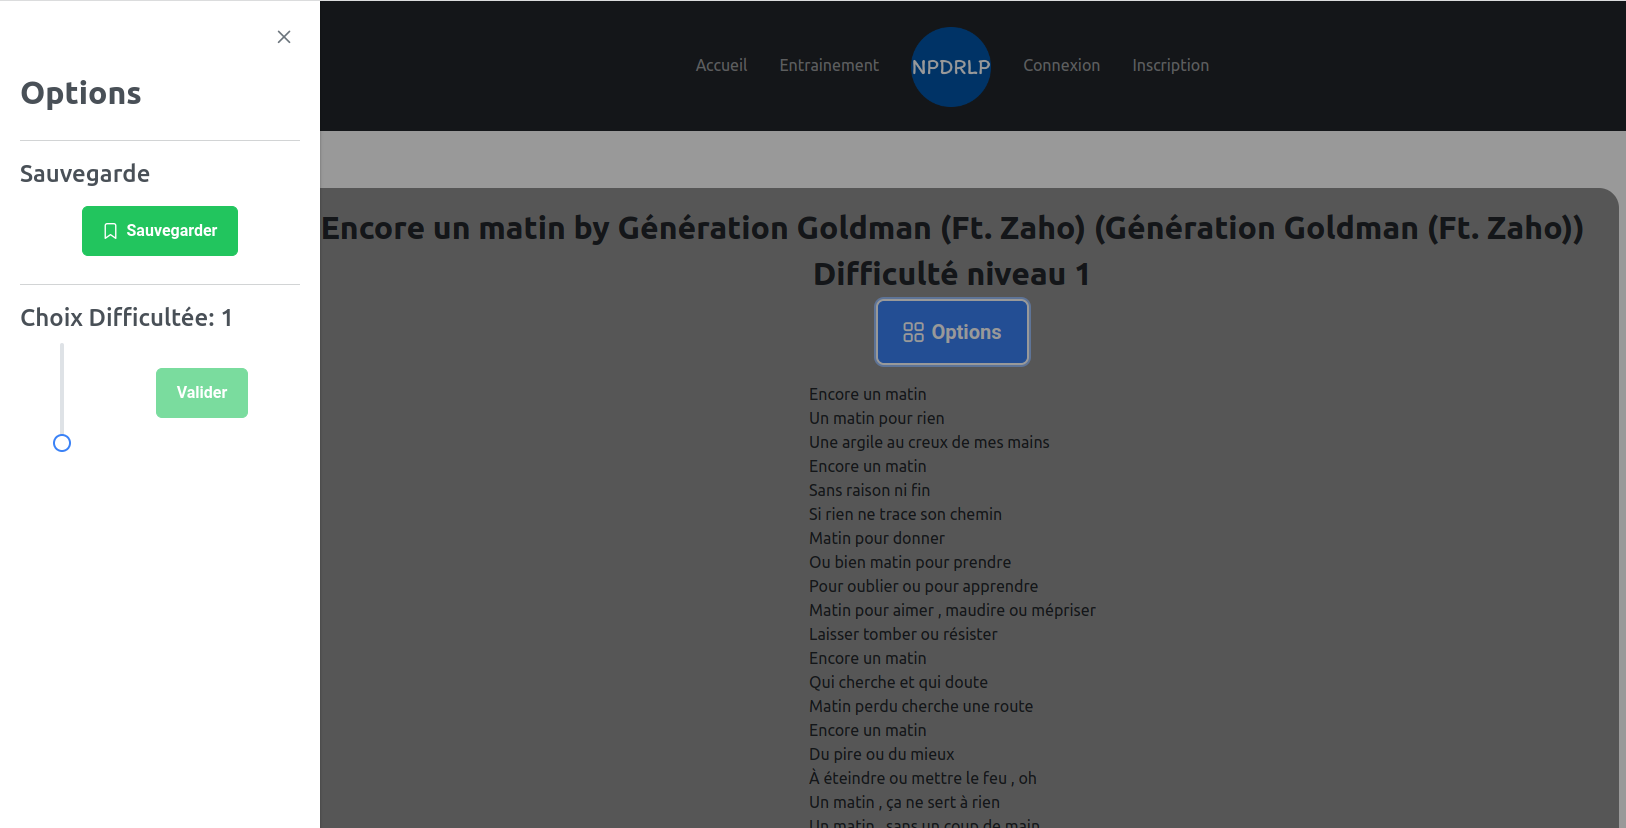
\includegraphics[scale=0.25]{optionparole.png}
	\caption{Options du mode entraînement}
\end{figure}

\paragraph{Sauvegarder la musique dans un dossier \\\\}

Lorsque vous cliquez sur le bouton "Sauvegarder la musique", deux possibilités s'offrent à vous. Si vous n'êtes pas connecté, nous vous informons qu'il faut que vous le soyez si vous souhaitez sauvegarder une musique. Sinon, une liste déroulante de tous vos dossiers apparaît, il suffit de cliquer sur le dossier dans lequel vous voulez sauvegarder la musique pour lancer la phase de sauvegarde.

Après ce clic, une pop-up apparaît vous demandant de confirmer votre choix. Lorsque cela est fait, une notification apparaît en haut à droite de votre écran vous informant que la sauvegarde a été effectuée !

\paragraph{Changer la difficulté \\\\}

Un curseur vertical vous permet de changer la difficulté. Selon la difficulté choisie, allant de 1 à 4, un certain nombre de trous vont apparaître dans les paroles de la musique et le but de l'utilisateur est de les compléter. Un bouton "Valider" apparaît aussi en bas des paroles afin d'effectuer une correction de vos réponses. Si la réponse est juste, la case se colore en vert et vous ne pouvez plus modifier votre réponse. Si elle est rouge, c'est que c'est faux.

Vous pouvez voir au-dessus des paroles un avancement du nombre de réponses justes par rapport au nombre de réponses attendues.

À noter que les trous sont disposés aléatoirement. Si jamais vous modifiez la difficulté, un nouveau pattern de trous sera appliqué aléatoirement.

\begin{figure}[H]
	\centering
	\begin{minipage}{.5\textwidth}
		\centering
		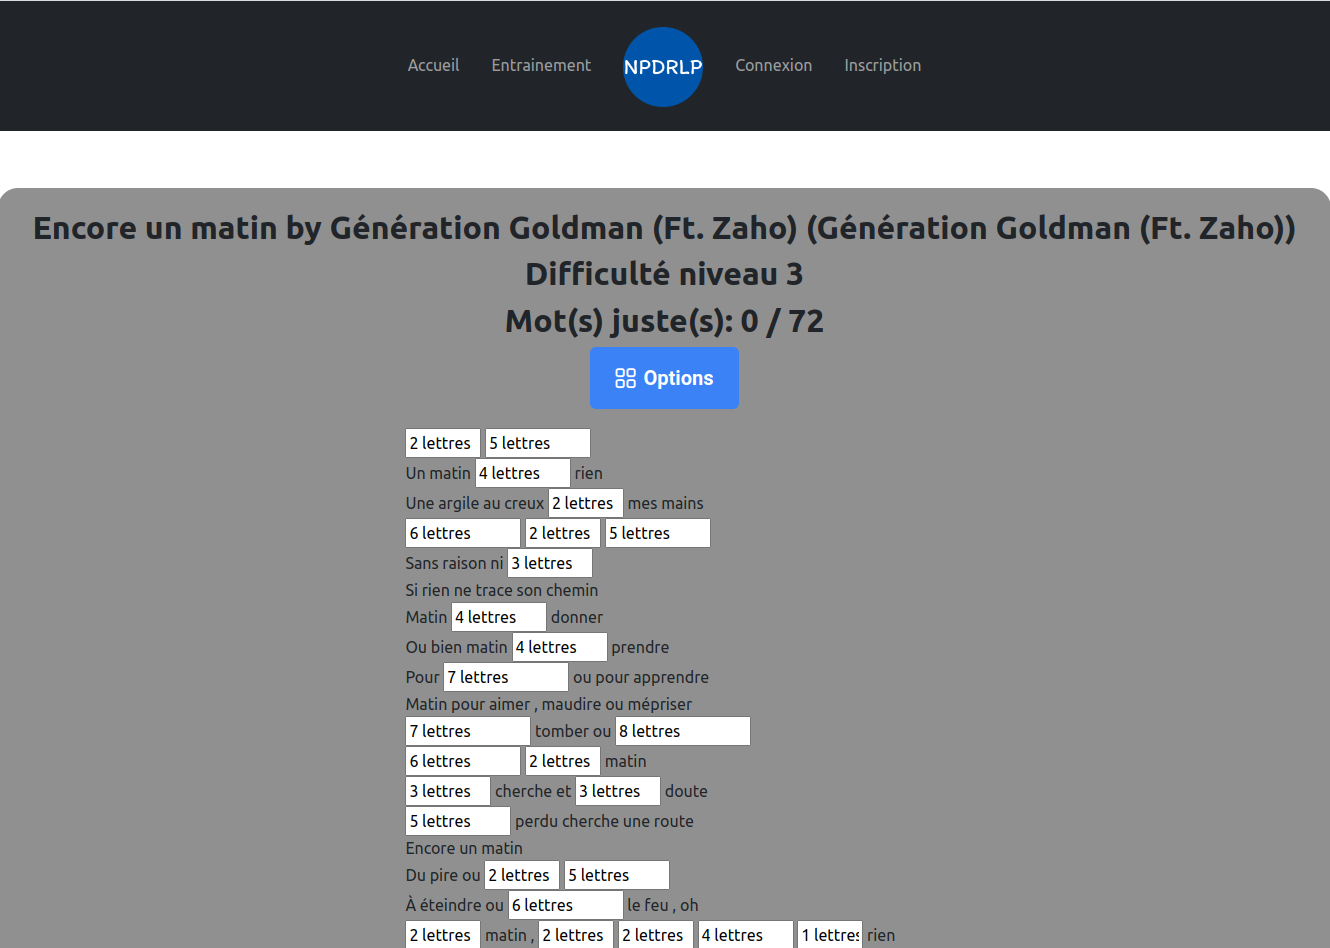
\includegraphics[scale=0.15]{diffi1.png}
	\end{minipage}%
	\begin{minipage}{.5\textwidth}
		\centering
		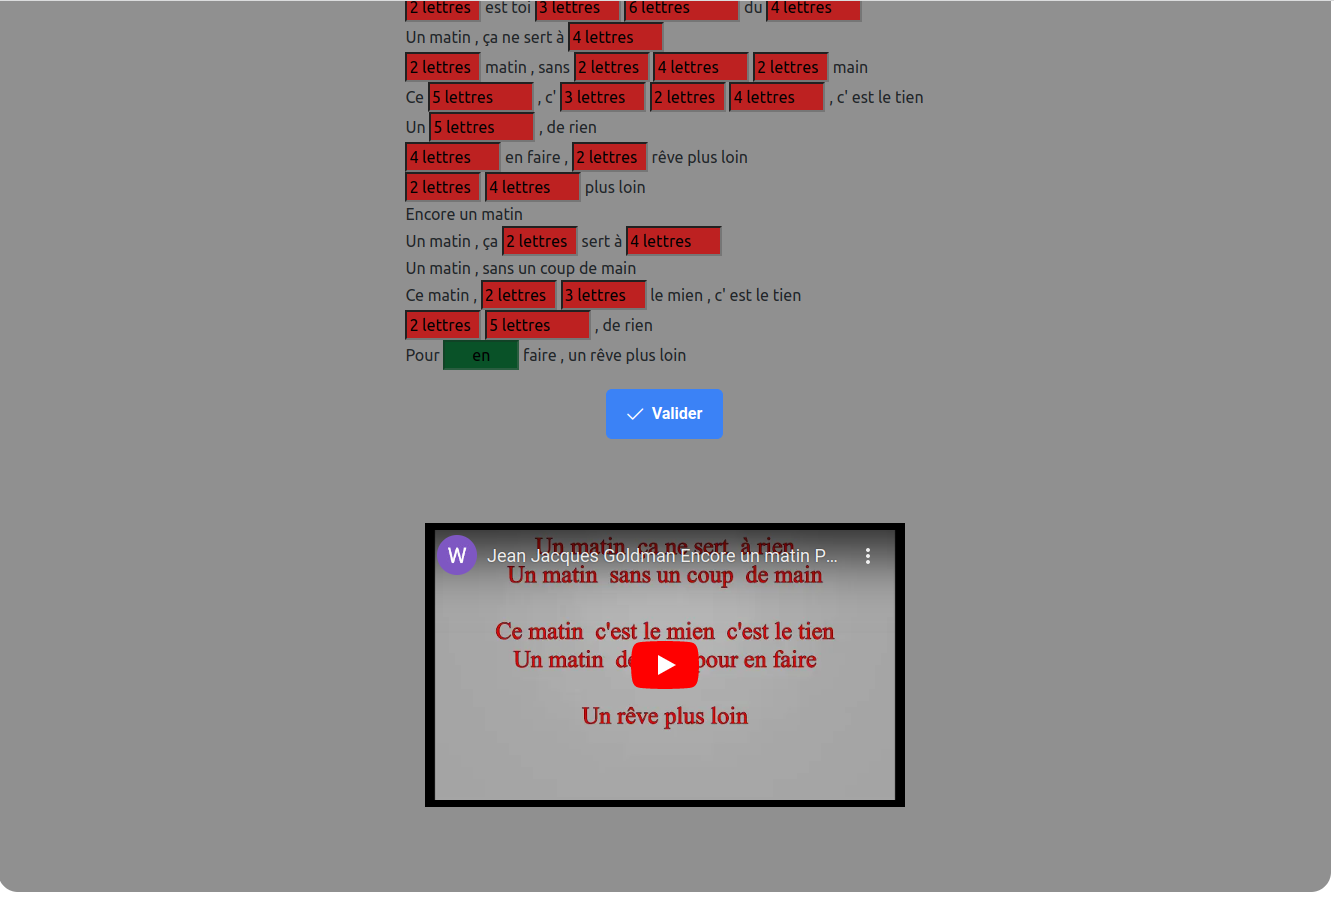
\includegraphics[scale=0.15]{diffi2.png}
	\end{minipage}
	\caption{Paroles avec des trous}
\end{figure}

\subsubsection{Inscription}

Lors de votre arrivée sur la page d'inscription, un formulaire est à remplir avec un nom d'utilisateur et une double vérification de mot de passe.

Lorsque l'utilisateur appuie sur le bouton "S'inscrire", plusieurs éléments sont vérifiés:

\begin{itemize}
	\item Nous vérifions déjà côté client que les deux mots de passe entrés sont identiques, sinon nous mettons un message d'erreur
	\item Ensuite, nous envoyons les informations au serveur. Deux retours sont alors possibles:
	\begin{itemize}
		\item Le nom d'utilisateur est déjà utilisé: on met un message d'erreur
		\item Nous avons bien enregistré le nouvel utilisateur
	\end{itemize}
\end{itemize}

\medskip

Si l'inscription a réussi, un message nous l'informe et nous sommes automatiquement redirigés vers la page de connexion après 5 secondes.

\begin{figure}[H]
	\centering
	\begin{minipage}{.5\textwidth}
		\centering
		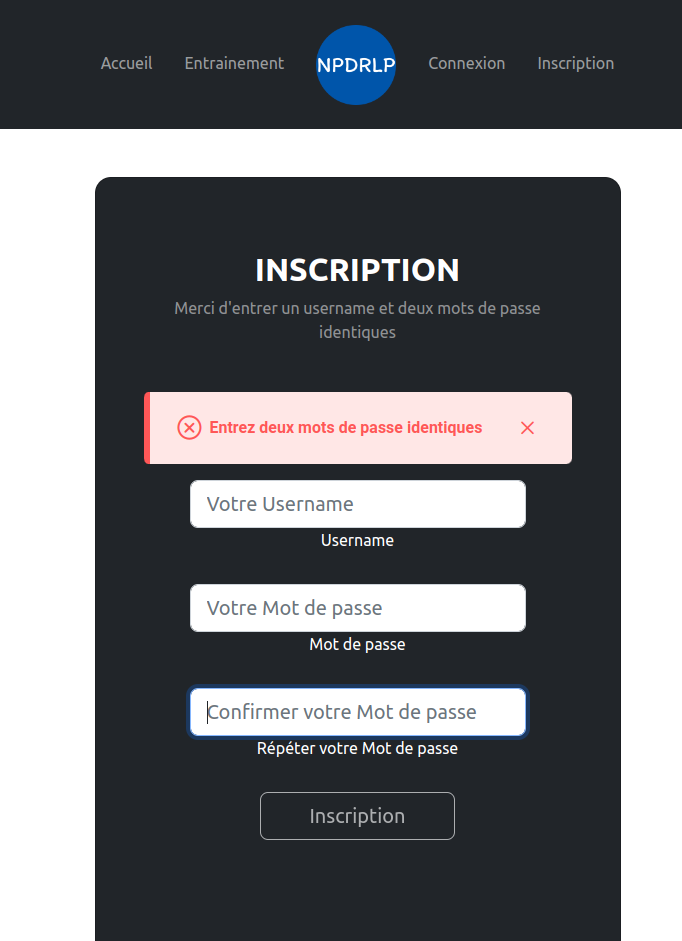
\includegraphics[scale=0.25]{inscri1.png}
	\end{minipage}%
	\begin{minipage}{.5\textwidth}
		\centering
		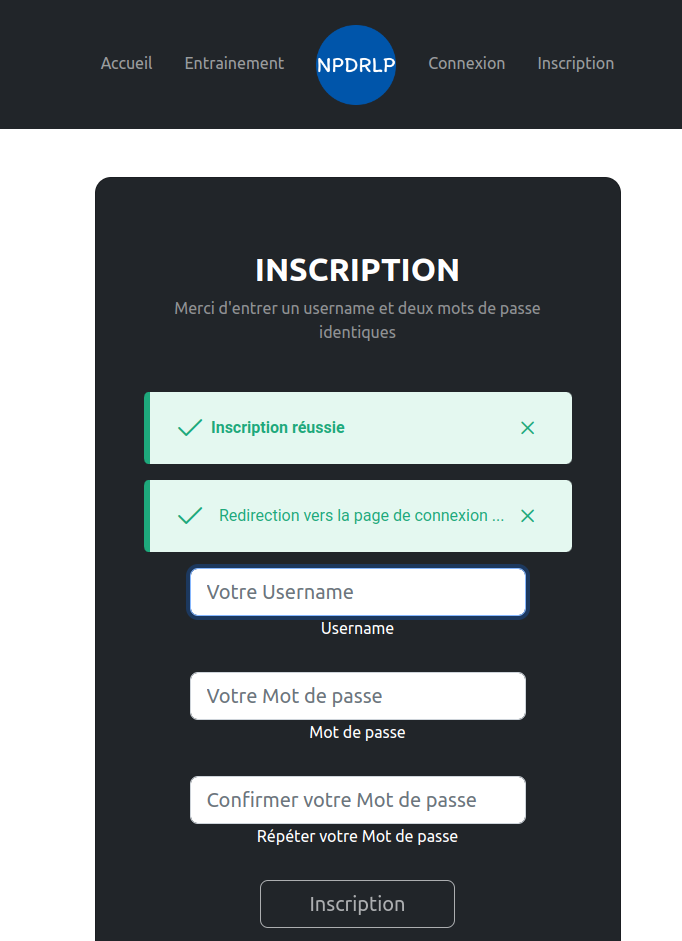
\includegraphics[scale=0.25]{inscri2.png}
	\end{minipage}
	\caption{Page d'inscription}
\end{figure}

\subsubsection{Connexion}

Nous avons ensuite la page de connexion. C'est ici que l'utilisateur, après s'être inscrit, va pouvoir débloquer l'accès à son menu personnel.

On demande de renseigner un nom d'utilisateur et le mot de passe qui va de pair avec.

Plusieurs cas d'erreur peuvent alors survenir:

\begin{itemize}
	\item Le nom d'utilisateur n'existe pas
	\item Le nom d'utilisateur existe mais le mot de passe est erroné
\end{itemize}

\medskip

Dans tous les cas, si une erreur a lieu, on empêche la connexion de l'utilisateur et on l'informe de l'erreur qui est survenue.

\begin{figure}[H]
	\centering
	\begin{minipage}{.5\textwidth}
		\centering
		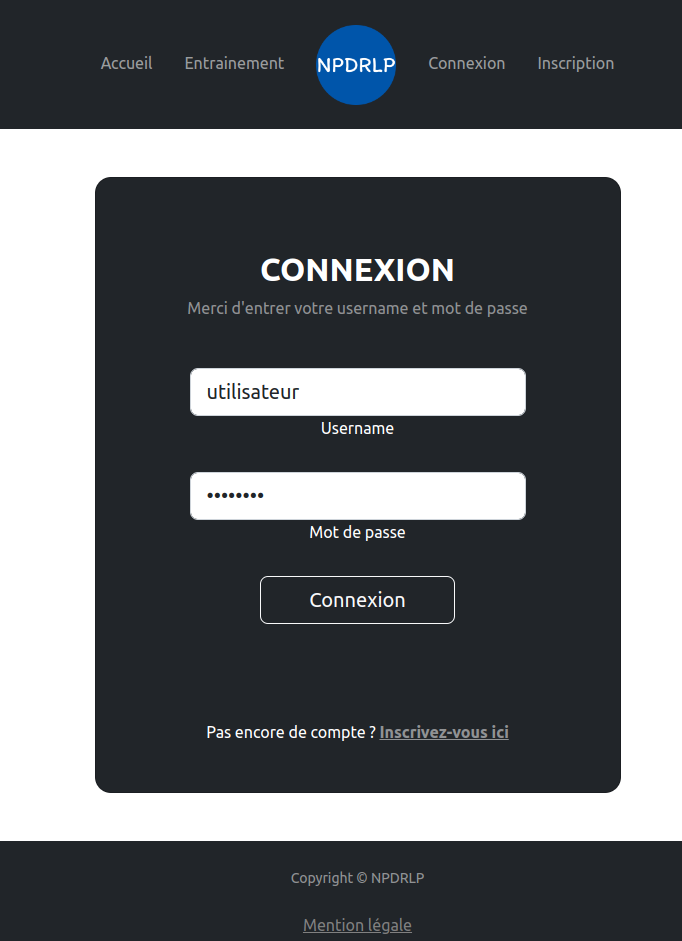
\includegraphics[scale=0.25]{connec1.png}
	\end{minipage}%
	\begin{minipage}{.5\textwidth}
		\centering
		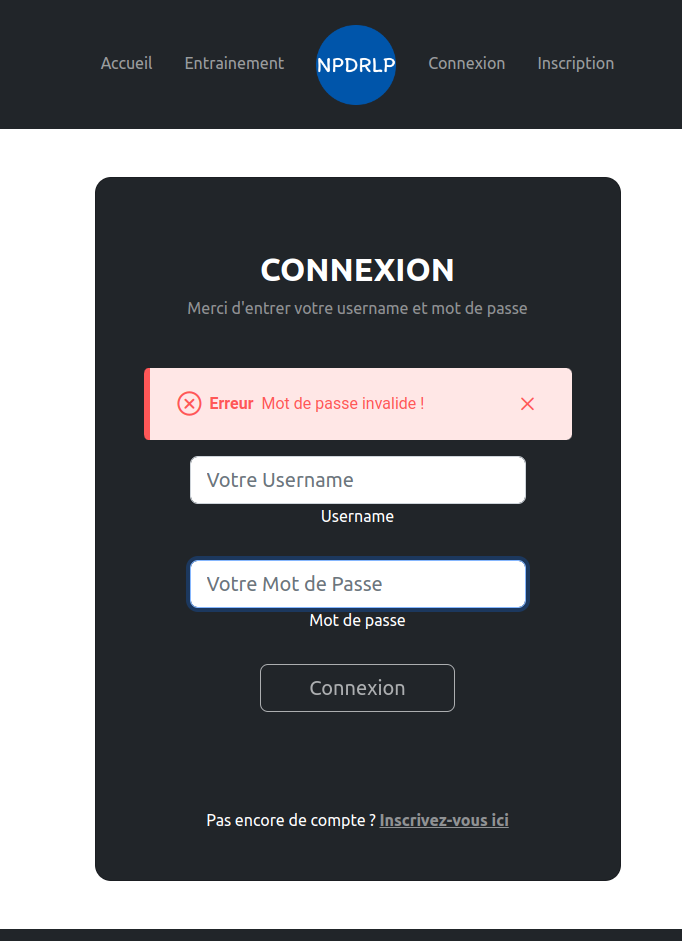
\includegraphics[scale=0.25]{connec2.png}
	\end{minipage}
	\caption{Page de connexion}
\end{figure}

Au contraire, si la connexion est réussie, on redirige automatiquement l'utilisateur vers sa page de menu. Cela arrivera quoi qu'il arrive : si jamais un utilisateur connecté essaye de retourner sur la page de connexion, nous le redirigeons directement vers son menu car il est déjà connecté !

\subsubsection{Menu de l'utilisateur}

Enfin, nous avons le menu de l'utilisateur.

Nous avons placé dedans un système d'édition de dossier ainsi qu'une explication brève et simple de comment fonctionne le site.

\begin{figure}[H]
	\centering
	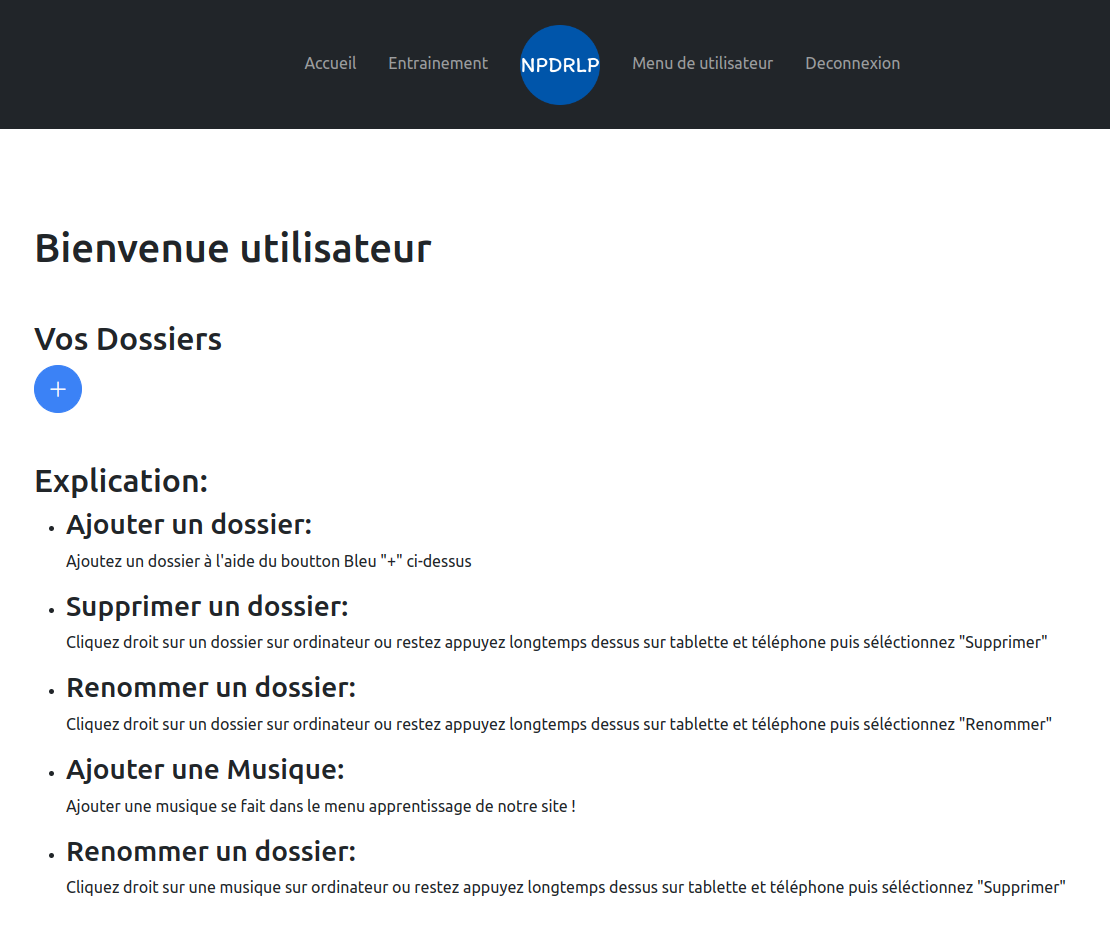
\includegraphics[scale=0.21]{menu.png}
	\caption{Le menu utilisateur}
\end{figure}

\paragraph{Le système d'édition de dossier \\\\}

À la première connexion, vous trouverez seulement un bouton avec le symbole "\textbf{+}". Ce bouton vous permet de créer un dossier avec le nom que vous voulez.

\begin{figure}[H]
	\centering
	\begin{minipage}{.5\textwidth}
		\centering
		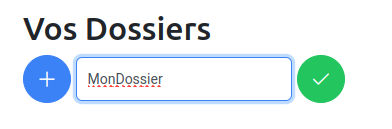
\includegraphics[scale=0.4]{dossier1.png}
	\end{minipage}%
	\begin{minipage}{.5\textwidth}
		\centering
		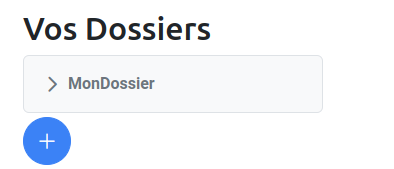
\includegraphics[scale=0.4]{dossier2.png}
	\end{minipage}
	\caption{Création d'un dossier}
\end{figure}

Vous avez ensuite la possibilité d'ajouter une musique dans un dossier comme expliqué plus tôt dans le mode entraînement.

Vous avez enfin la possibilité d'éditer vos dossiers. En faisant sur votre ordinateur un clic droit (ou un clic long sur votre téléphone et tablette) sur un dossier, vous pouvez soit le supprimer lui et toutes les musiques qui le composent, soit le renommer.

Si vous faites un clic droit sur une musique, vous pouvez la supprimer.

Avant chaque suppression d'un élément, nous demandons une confirmation à l'utilisateur car cette action est irrévocable. Une notification vous informe si votre action a bien été prise en compte ou non en haut à droite de votre écran.


\begin{figure}[H]
	\centering
	\begin{minipage}{.3\textwidth}
		\centering
		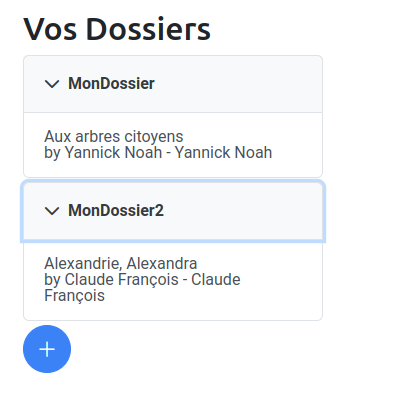
\includegraphics[scale=0.4]{dossier3.png}
	\end{minipage}%
	\begin{minipage}{.3\textwidth}
		\centering
		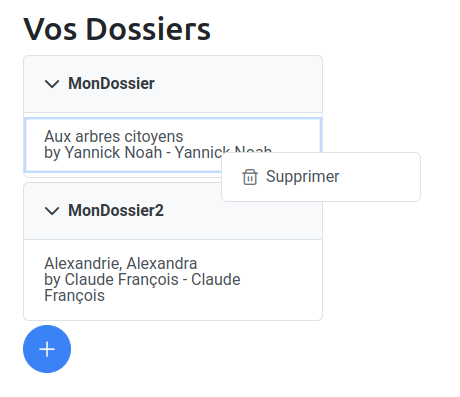
\includegraphics[scale=0.4]{dossier4.png}
	\end{minipage}
\begin{minipage}{.3\textwidth}
	\centering
	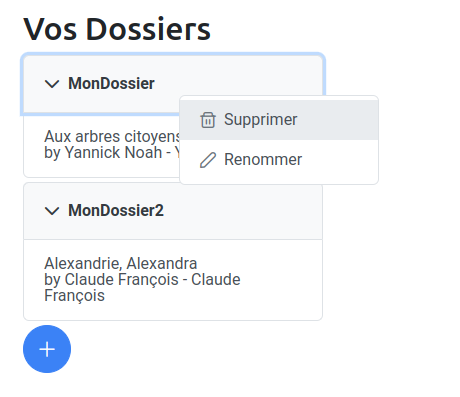
\includegraphics[scale=0.4]{dossier5.png}
\end{minipage}
	\caption{Édition des dossiers et musiques}    
\end{figure}

\newpage
\vspace*{1cm}

\subsection{Discussions et perspectives}

Maintenant que notre projet est terminé, nous nous posons les deux questions habituelles à se poser à la fin d'un projet. La première est : 
\newline

- Si nous recommencions les projet que ferions nous de mieux ?  
\newline


Pour nous, la conception et l'implémentation de notre projet s'est passée à peu de choses près comme nous l'avions espéré. Nous n'avons pas manqué de temps car notre planning anticipé nous a aidé à appréhender les problèmes à analyser, et la gestion de projet nous a grandement aidés dans ce domaine. Néanmoins, la seule fonctionnalité manquante de notre Gantt prévisionnel est le format karaoké à proprement parlé de notre application. Suite aux difficultés et à l'innovation que cela représentait de créer un algorithme capable d'écrire les paroles en fonction de la musique, nous nous sommes rabattus sur l'\gls{API} YouTube en obtenant un karaoké déjà existant. Le produit que nous considérons comme "livré" correspond donc totalement à nos attentes de début de projet car celui-ci s'est bien déroulé.La deuxième question que l'on se pose régulièrement après un projet est :
\newline

- Qu'envisageriez vous de rajouter à votre projet ?
\newline

Dans un premier temps, le projet nous intéressant énormément, nous avions pour objectif de publier ce site web en louant notre nom de domaine pour permettre aux gens de pouvoir réviser pour l'émission "N'oubliez pas les paroles" sans soucis. Cela nous aurait donc forcé à trouver une autre solution que les \gls{Web scraping} utilisés pour récupérer les paroles de n'importe quelle chanson, mais aussi de voir avec des organismes comme la \gls{SACEM} pour acheter les droits d'exploitation des musiques pour notre site.

Enfin, ce concept de site n'existant pas encore pour participer à "N'oubliez pas les paroles", nous pourrions proposer à France Télévision un partenariat pour permettre à notre site d'avoir de la visibilité et à leur émission d'avoir du renouveau.

\newpage
\vspace*{1cm}

\section*{Conclusion}
\addcontentsline{toc}{section}{\protect\numberline{}Conclusion}

En conclusion, la réalisation de ce projet a été une expérience enrichissante pour notre équipe. Nous avons réussi à créer une application web qui répond à un besoin précis et qui offre des fonctionnalités avancées pour l'apprentissage de la musique. La gestion de la base de données et la création de l'interface utilisateur ont été des aspects clés de notre projet.

\medskip

Au niveau technique, nous avons utilisé différentes technologies pour concevoir notre application. Nous avons choisi de travailler avec Angular pour la partie \gls{Front} de notre application, qui nous a permis de créer une interface utilisateur dynamique et réactive. Pour la gestion de la base de données, nous avons utilisé SQLPlus et MySQL Workbench, deux outils puissants pour la gestion de bases de données relationnelles. Nous avons également utilisé Bootstrap et PrimeNG pour le design et le style de notre application.

\medskip

La réalisation de ce projet nous a permis de mettre en pratique nos compétences en développement web et en gestion de projets. Nous avons dû faire face à plusieurs défis, tels que la gestion des conflits de versions et la coordination de l'équipe pour respecter les délais fixés. Nous avons également appris à travailler en équipe et à communiquer efficacement pour assurer le bon déroulement du projet.

\medskip

Enfin, nous sommes satisfaits du résultat final de notre application. Nous pensons que celle-ci pourrait être utile pour les personnes souhaitant apprendre la musique de manière interactive et efficace. Nous sommes conscients qu'il reste des améliorations à apporter et des fonctionnalités à ajouter pour améliorer l'expérience utilisateur et la performance de l'application. Nous sommes donc ouverts à toute suggestion d'amélioration pour cette application dans le futur.

\newpage
\vspace*{1cm}

\section*{Références bibliographiques}
\addcontentsline{toc}{section}{\protect\numberline{}Référence bibliographique}

[\textbf{Node.js}] \href{https://nodejs.org/}{https://nodejs.org/} (17/11/2022) \newline\newline
[\textbf{NPM Express}] \href{https://www.npmjs.com/package/express}{https://www.npmjs.com/package/express} (28/11/2022)\newline\newline
[\textbf{NPM}] \href{https://www.npmjs.com/}{https://www.npmjs.com/} (18/11/2022)\newline\newline
[\textbf{Angular}] \href{https://angular.io/}{https://angular.io/} (22/11/2022)\newline\newline
[\textbf{Bootstrap}] \href{https://getbootstrap.com/}{https://getbootstrap.com/} (08/02/2023)\newline\newline
[\textbf{PrimeNG}] \href{https://www.primefaces.org/primeng/}{https://www.primefaces.org/primeng/} (03/12/2022)\newline\newline
[\textbf{MySql}] \href{https://www.mysql.com/fr/}{https://www.mysql.com/fr/} (23/12/2022)\newline\newline
[\textbf{API YouTube Data API v3}] \href{https://developers.google.com/youtube/v3}{https://developers.google.com/youtube/v3} (12/02/2023) \newline\newline
[\textbf{API ChartLyrics}] \href{https://www.chartlyrics.com/}{https://www.chartlyrics.com/} (29/11/2022)\newline\newline
[\textbf{API Genius Lyrics}] \href{https://docs.genius.com/}{https://docs.genius.com/} (30/11/2022)\newline\newline
[\textbf{Journal du net}] \href{https://www.journaldunet.fr/}{https://www.journaldunet.fr/} (12/02/2023)\newline


\addcontentsline{toc}{section}{\protect\numberline{}Glossaire}

\printglossary[type=main, title=Glossaire]


\end{document}
